\documentclass[11pt,a4paper]{article}
\usepackage[utf8]{inputenc}
\usepackage[T1]{fontenc}
\usepackage[top=2.5cm, bottom=2.5cm, left=2.5cm, right=2.5cm]{geometry}
\usepackage{graphicx}
\usepackage{float}
\usepackage{xcolor}
\usepackage{titlesec}
\usepackage{fancyhdr}
\usepackage{hyperref}
\usepackage{booktabs}
\usepackage{tabularx}
\usepackage{colortbl}
\usepackage{enumitem}
\usepackage{tcolorbox}
\usepackage{amsmath}
\usepackage{subcaption}

\tcbuselibrary{skins,breakable,raster}

% ── Paleta BlackLine (dark luxury) ──────────────────────────────────────────
\definecolor{blkGold}{HTML}{D4A843}
\definecolor{blkDark}{HTML}{0D0D0D}
\definecolor{blkCard}{HTML}{1A1A1A}
\definecolor{blkMid}{HTML}{2A2A2A}
\definecolor{blkText}{HTML}{E0E0E0}
\definecolor{blkGreen}{HTML}{22C55E}
\definecolor{blkRed}{HTML}{EF4444}
\definecolor{blkBlue}{HTML}{3B82F6}

% ── Configuración de página ───────────────────────────────────────────────
\pagecolor{blkDark}
\color{blkText}

% ── Encabezado/pie ────────────────────────────────────────────────────────
\pagestyle{fancy}
\fancyhf{}
\fancyhead[L]{\textcolor{blkGold}{\small\textbf{BlackLine}}}
\fancyhead[R]{\textcolor{blkGold}{\small Documentación Técnica de Algoritmos}}
\fancyfoot[C]{\textcolor{blkGold}{\small\thepage}}
\renewcommand{\headrulewidth}{0.4pt}
\renewcommand{\headrule}{\hbox to\headwidth{\color{blkGold}\leaders\hrule height \headrulewidth\hfill}}

% ── Secciones con acento dorado ──────────────────────────────────────────
\titleformat{\section}
  {\large\bfseries\color{blkGold}}
  {\thesection.}{0.8em}{}[\color{blkGold}\titlerule]
\titleformat{\subsection}
  {\normalsize\bfseries\color{blkText}}
  {\thesubsection.}{0.6em}{}

\titlespacing*{\section}{0pt}{16pt}{8pt}
\titlespacing*{\subsection}{0pt}{10pt}{4pt}

% ── Cajas de información ─────────────────────────────────────────────────
\tcbset{
  infobox/.style={
    colback=blkCard, colframe=blkGold, coltext=blkText,
    fonttitle=\bfseries\color{blkGold},
    boxrule=0.6pt, arc=4pt,
    left=8pt, right=8pt, top=6pt, bottom=6pt
  },
  codebox/.style={
    colback=blkMid, colframe=blkBlue!60, coltext=blkText,
    fonttitle=\bfseries\small\color{blkBlue!80},
    boxrule=0.5pt, arc=3pt,
    left=6pt, right=6pt, top=4pt, bottom=4pt,
    fontupper=\ttfamily\small
  },
  rulebox/.style={
    colback=blkCard, colframe=blkGreen!70, coltext=blkText,
    fonttitle=\bfseries\color{blkGreen},
    boxrule=0.5pt, arc=3pt,
    left=8pt, right=8pt, top=6pt, bottom=6pt
  },
  warnbox/.style={
    colback=blkCard, colframe=blkRed!70, coltext=blkText,
    fonttitle=\bfseries\color{blkRed},
    boxrule=0.5pt, arc=3pt,
    left=8pt, right=8pt, top=6pt, bottom=6pt
  }
}

% ── hyperref oscuro ────────────────────────────────────────────────────────
\hypersetup{
  colorlinks=true,
  linkcolor=blkGold,
  urlcolor=blkBlue!80,
  pdfborder={0 0 0}
}

% ── Tablas ────────────────────────────────────────────────────────────────
\arrayrulecolor{blkGold}
\setlength{\arrayrulewidth}{0.4pt}

\begin{document}

% ── PORTADA ────────────────────────────────────────────────────────────────
\begin{titlepage}
  \centering
  \vspace*{3cm}
  {\fontsize{36}{44}\selectfont\bfseries\color{blkGold} BlackLine}\\[0.4cm]
  {\large\color{blkText!70} Tattoo \& Piercing Marketplace}\\[2.5cm]
  {\fontsize{22}{28}\selectfont\bfseries\color{blkText}
    Documentación Técnica\\[0.3cm]
    de Algoritmos Core}\\[1.2cm]
  \textcolor{blkGold}{\rule{0.5\textwidth}{0.8pt}}\\[1.5cm]
  {\normalsize\color{blkText!70}
    \begin{tabular}{rl}
      \textcolor{blkGold}{Versión:}    & 2.0.0\\[4pt]
      \textcolor{blkGold}{Fecha:}      & Mayo 2026\\[4pt]
      \textcolor{blkGold}{Stack:}      & Django REST + Angular 19 + PostgreSQL\\[4pt]
      \textcolor{blkGold}{Rama:}       & BL-95-RF-4 (Contraoferta de precio/fecha)\\
    \end{tabular}
  }\\[2.5cm]
  \textcolor{blkGold}{\rule{0.5\textwidth}{0.8pt}}\\[1cm]
  {\small\color{blkText!50}
    Este documento describe los algoritmos, flujos de datos y\\
    decisiones arquitectónicas centrales del sistema BlackLine.
  }
  \vfill
  {\footnotesize\color{blkText!40} Generado con \texttt{claude-sonnet-4-6} · BlackLine Engineering}
\end{titlepage}

% ── TABLA DE CONTENIDOS ────────────────────────────────────────────────────
\tableofcontents
\clearpage

% ────────────────────────────────────────────────────────────────────────────
\section{Visión General de la Arquitectura}
% ────────────────────────────────────────────────────────────────────────────

BlackLine sigue una arquitectura \textbf{SPA + REST API} con separación estricta de
responsabilidades entre frontend y backend.

\begin{tcbitemize}[raster columns=2, raster equal height,
  colback=blkCard, colframe=blkGold!50, arc=4pt, boxrule=0.5pt,
  fontupper=\small\color{blkText}]
\tcbitem[title={\textcolor{blkGold}{Frontend (Angular 19)}}]
  \begin{itemize}[leftmargin=12pt, itemsep=2pt]
    \item Componentes por feature module
    \item Signals + NgRx para estado reactivo
    \item Guards e interceptores HTTP
    \item Tipos generados desde OpenAPI
  \end{itemize}
\tcbitem[title={\textcolor{blkGold}{Backend (Django REST)}}]
  \begin{itemize}[leftmargin=12pt, itemsep=2pt]
    \item ViewSets + Serializers (DRF)
    \item Servicios de lógica de negocio
    \item Modelos ORM con PostgreSQL
    \item JWT con SimpleJWT
  \end{itemize}
\end{tcbitemize}

\begin{tcolorbox}[infobox, title={Contrato API}]
Toda respuesta sigue el contrato:
\begin{itemize}[itemsep=2pt]
  \item \textbf{Éxito:} \texttt{\{ data: T, message?: string \}}
  \item \textbf{Error:} \texttt{\{ data: null, errors: Record<string, string[]> \}}
  \item \textbf{Lista paginada:} \texttt{\{ count, next, previous, results: T[] \}}
\end{itemize}
\end{tcolorbox}

% ────────────────────────────────────────────────────────────────────────────
\section{Algoritmo de Precio Canónico}
% ────────────────────────────────────────────────────────────────────────────

\subsection{Descripción}

El cálculo de precio es la operación económica central del sistema. El backend
es la \textbf{única fuente de verdad}; el frontend muestra únicamente un rango estimado.

\subsection{Fórmula}

\begin{tcolorbox}[codebox, title={Fórmula canónica (backend/apps/quotes/views.py)}]
\texttt{estimated\_price = MAX(}\\
\texttt{\ \ \ \ size\_cm $\times$ base\_hourly\_rate $\times$ zone\_multiplier $\times$ color\_multiplier,}\\
\texttt{\ \ \ \ minimum\_setup\_fee}\\
\texttt{)}
\end{tcolorbox}

El rango que se muestra al cliente se calcula en el frontend:
\[
\text{price\_min} = \text{estimated\_price}, \qquad
\text{price\_max} = \text{estimated\_price} \times 1.35
\]
usando \texttt{BASE\_RATE\_MXN = 150} como tarifa de mercado promedio.

\subsection{Multiplicadores por zona corporal}

\begin{center}
\begin{tabular}{lc|lc}
\toprule
\rowcolor{blkMid}\textcolor{blkGold}{\textbf{Zona}} & \textcolor{blkGold}{\textbf{Factor}} &
\textcolor{blkGold}{\textbf{Zona}} & \textcolor{blkGold}{\textbf{Factor}}\\
\midrule
\texttt{BRAZO}      & 1.00 & \texttt{ESPALDA}   & 1.30\\
\rowcolor{blkMid}
\texttt{ANTEBRAZO}  & 1.00 & \texttt{PECHO}     & 1.25\\
\texttt{PIERNA}     & 1.10 & \texttt{COSTILLAS} & 1.50\\
\rowcolor{blkMid}
\texttt{HOMBRO}     & 1.05 & \texttt{CUELLO}    & 1.40\\
\texttt{MANO}       & 1.35 & \texttt{PIE}       & 1.35\\
\bottomrule
\end{tabular}
\end{center}

\textbf{Multiplicador de color:} $\times 1.20$ si \texttt{is\_color = true}, $\times 1.00$ si blanco y negro.

\begin{tcolorbox}[warnbox, title={Regla de sincronización}]
Los valores de \texttt{BODY\_PART\_MULTIPLIERS} en \texttt{backend/apps/quotes/views.py}
son la fuente de verdad. Si se modifican, deben actualizarse también en
\texttt{cotizador.component.ts}.
\end{tcolorbox}

\subsection{Diagrama de flujo}

\begin{figure}[H]
  \centering
  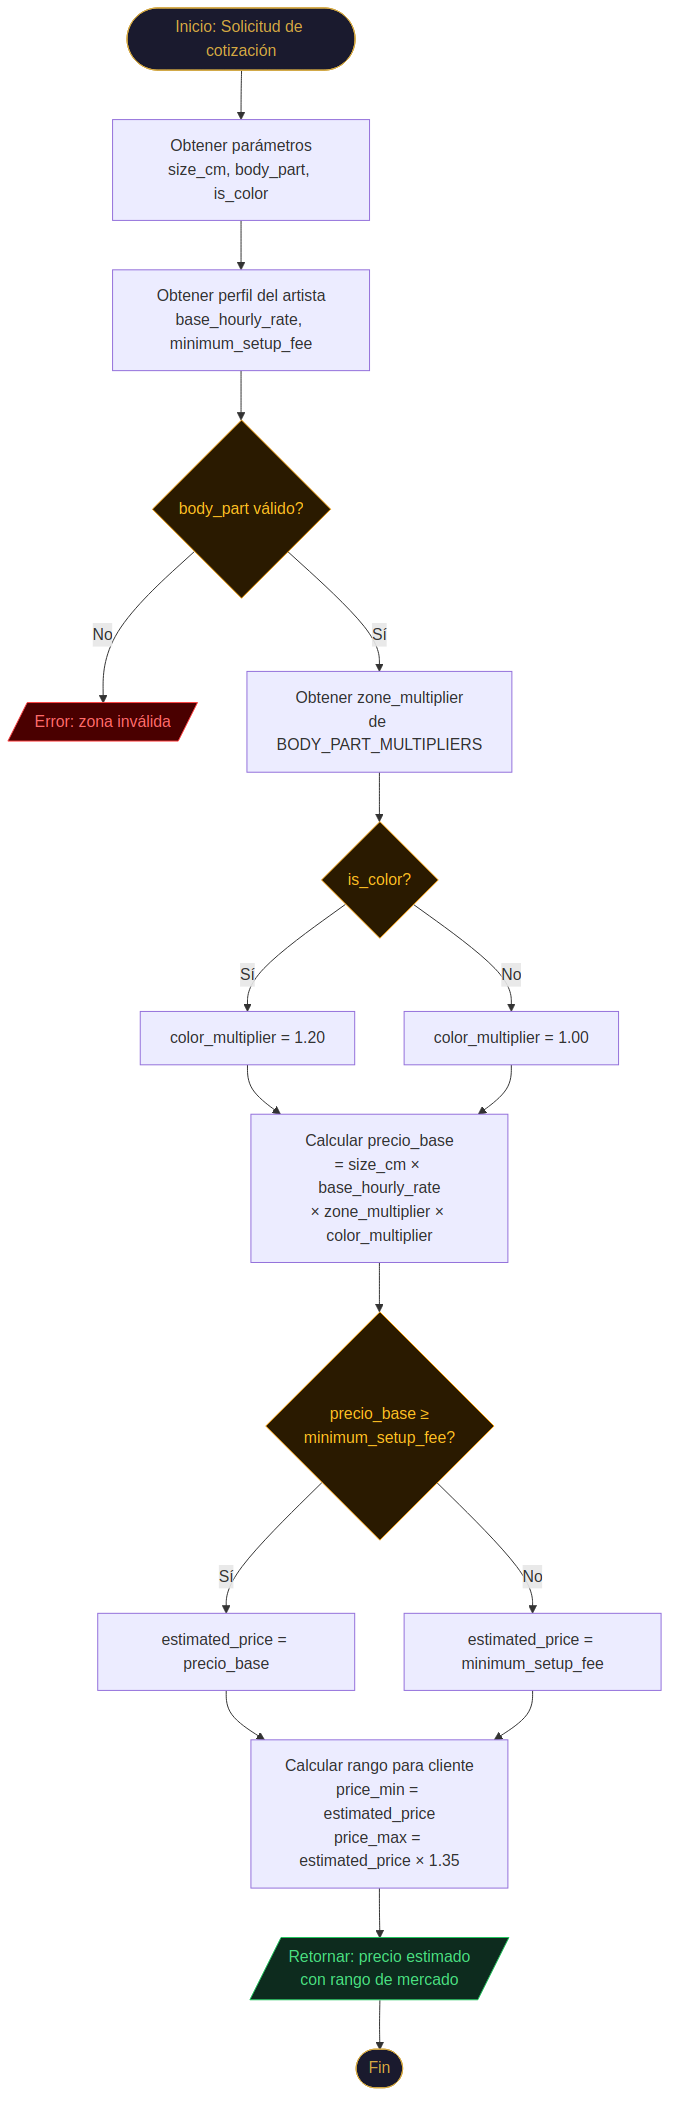
\includegraphics[width=0.78\textwidth]{../diagrams/generated/01_precio_canonico.png}
  \caption{Algoritmo de cálculo de precio estimado con multiplicadores de zona y color}
  \label{fig:precio}
\end{figure}

% ────────────────────────────────────────────────────────────────────────────
\section{Flujo Cotizador $\to$ Match $\to$ Cita}
% ────────────────────────────────────────────────────────────────────────────

\subsection{Descripción}

El flujo principal del cliente recorre tres etapas: creación de la solicitud de
cotización, búsqueda de artistas compatibles (match), y agendamiento de la cita.

\subsection{Gestión de estado en cliente}

\begin{tcolorbox}[codebox, title={QuoteService.lastQuote (Angular Signal)}]
\texttt{ngOnInit():}\\
\texttt{\ \ 1. Si lastQuote() $\to$ usa in-memory (restaurado desde sessionStorage)}\\
\texttt{\ \ 2. Si null $\to$ getMyQuotes() y carga la más reciente de la API}\\[4pt]
\texttt{setLastQuote(quote):}\\
\texttt{\ \ Escribe Signal + sessionStorage atómicamente}
\end{tcolorbox}

\subsection{Endpoints involucrados}

\begin{center}
\begin{tabularx}{0.9\textwidth}{llX}
\toprule
\rowcolor{blkMid}
\textcolor{blkGold}{\textbf{Método}} &
\textcolor{blkGold}{\textbf{Endpoint}} &
\textcolor{blkGold}{\textbf{Acción}}\\
\midrule
\texttt{POST} & \texttt{/api/quotes/} & Crea QuoteRequest\\
\rowcolor{blkMid}
\texttt{GET}  & \texttt{/api/quotes/match/} & Artistas filtrados por ciudad + estilo\\
\texttt{POST} & \texttt{/api/quotes/appointments/} & Crea Appointment (PENDING)\\
\rowcolor{blkMid}
\texttt{POST} & \texttt{/api/quotes/appointments/\{id\}/health-consent/} & Guarda HealthConsent\\
\bottomrule
\end{tabularx}
\end{center}

\subsection{Diagrama de secuencia}

\begin{figure}[H]
  \centering
  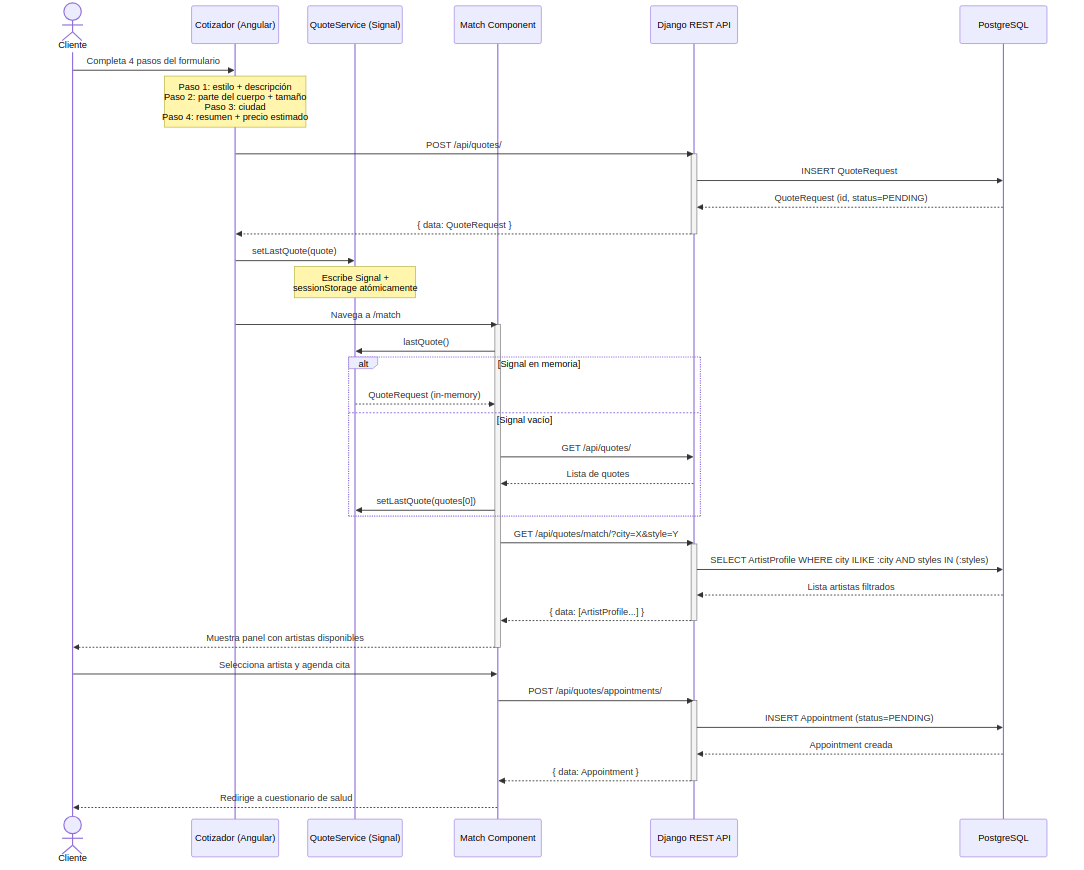
\includegraphics[width=0.92\textwidth]{../diagrams/generated/02_flujo_cotizador_match_cita.png}
  \caption{Secuencia completa: creación de cotización, búsqueda de artista y agendamiento de cita}
  \label{fig:cotizador}
\end{figure}

% ────────────────────────────────────────────────────────────────────────────
\section{Máquina de Estados de la Cita}
% ────────────────────────────────────────────────────────────────────────────

\subsection{Descripción}

Las citas (\texttt{Appointment}) siguen una máquina de estados estricta. Solo el
artista puede iniciar transiciones desde \texttt{PENDING}.

\subsection{Transiciones válidas}

\begin{center}
\begin{tabular}{lll}
\toprule
\rowcolor{blkMid}
\textcolor{blkGold}{\textbf{Estado origen}} &
\textcolor{blkGold}{\textbf{Estado destino}} &
\textcolor{blkGold}{\textbf{Condición}}\\
\midrule
\texttt{PENDING}       & \texttt{APPROVED}      & Artista acepta cita\\
\rowcolor{blkMid}
\texttt{PENDING}       & \texttt{REJECTED}      & Artista rechaza cita\\
\texttt{PENDING}       & \texttt{COUNTER\_OFFER}& Artista propone cambios\\
\rowcolor{blkMid}
\texttt{COUNTER\_OFFER}& \texttt{APPROVED}      & Cliente acepta contraoferta\\
\texttt{COUNTER\_OFFER}& \texttt{REJECTED}      & Cliente rechaza contraoferta\\
\bottomrule
\end{tabular}
\end{center}

\begin{tcolorbox}[infobox, title={Endpoint de transición}]
\texttt{PATCH /api/quotes/appointments/\{id\}/status/}\\[4pt]
Body para contraoferta: \texttt{\{ "status": "COUNTER\_OFFER", "price": 1500, "scheduled\_at": "..." \}}
\end{tcolorbox}

\subsection{Diagrama de estados}

\begin{figure}[H]
  \centering
  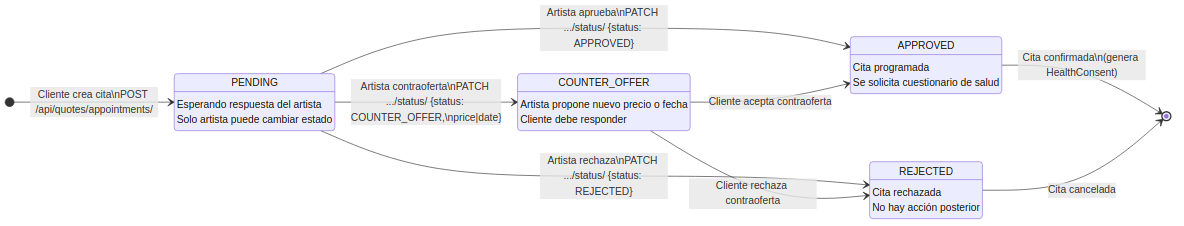
\includegraphics[width=0.88\textwidth]{../diagrams/generated/03_maquina_estados_cita.png}
  \caption{Máquina de estados de Appointment: transiciones y actores responsables}
  \label{fig:estados}
\end{figure}

% ────────────────────────────────────────────────────────────────────────────
\section{Gestión de Sesión JWT}
% ────────────────────────────────────────────────────────────────────────────

\subsection{Descripción}

El sistema usa JWT con rotación de refresh tokens. El interceptor HTTP gestiona
automáticamente la renovación transparente para el usuario.

\subsection{Reglas de seguridad}

\begin{tcolorbox}[warnbox, title={Política de almacenamiento (OWASP)}]
\begin{itemize}[itemsep=3pt]
  \item \textbf{PERMITIDO:} \texttt{sessionStorage} — se limpia al cerrar el navegador
  \item \textbf{PROHIBIDO:} \texttt{localStorage} — persiste entre sesiones, riesgo XSS
  \item Los tokens se eliminan completamente en \texttt{logout()}
  \item El refresh token se invalida en el backend (blacklist)
\end{itemize}
\end{tcolorbox}

\subsection{Flujo de renovación automática}

Cuando el servidor retorna \texttt{401 Unauthorized}, el \texttt{JwtInterceptor} realiza
automáticamente:
\begin{enumerate}[itemsep=4pt]
  \item Recupera el refresh token de \texttt{sessionStorage}
  \item Llama a \texttt{POST /api/auth/token/refresh/}
  \item Almacena el nuevo access token
  \item Reintenta la petición original con el token renovado
  \item Si el refresh también falla, redirige al login
\end{enumerate}

\subsection{Diagrama de secuencia}

\begin{figure}[H]
  \centering
  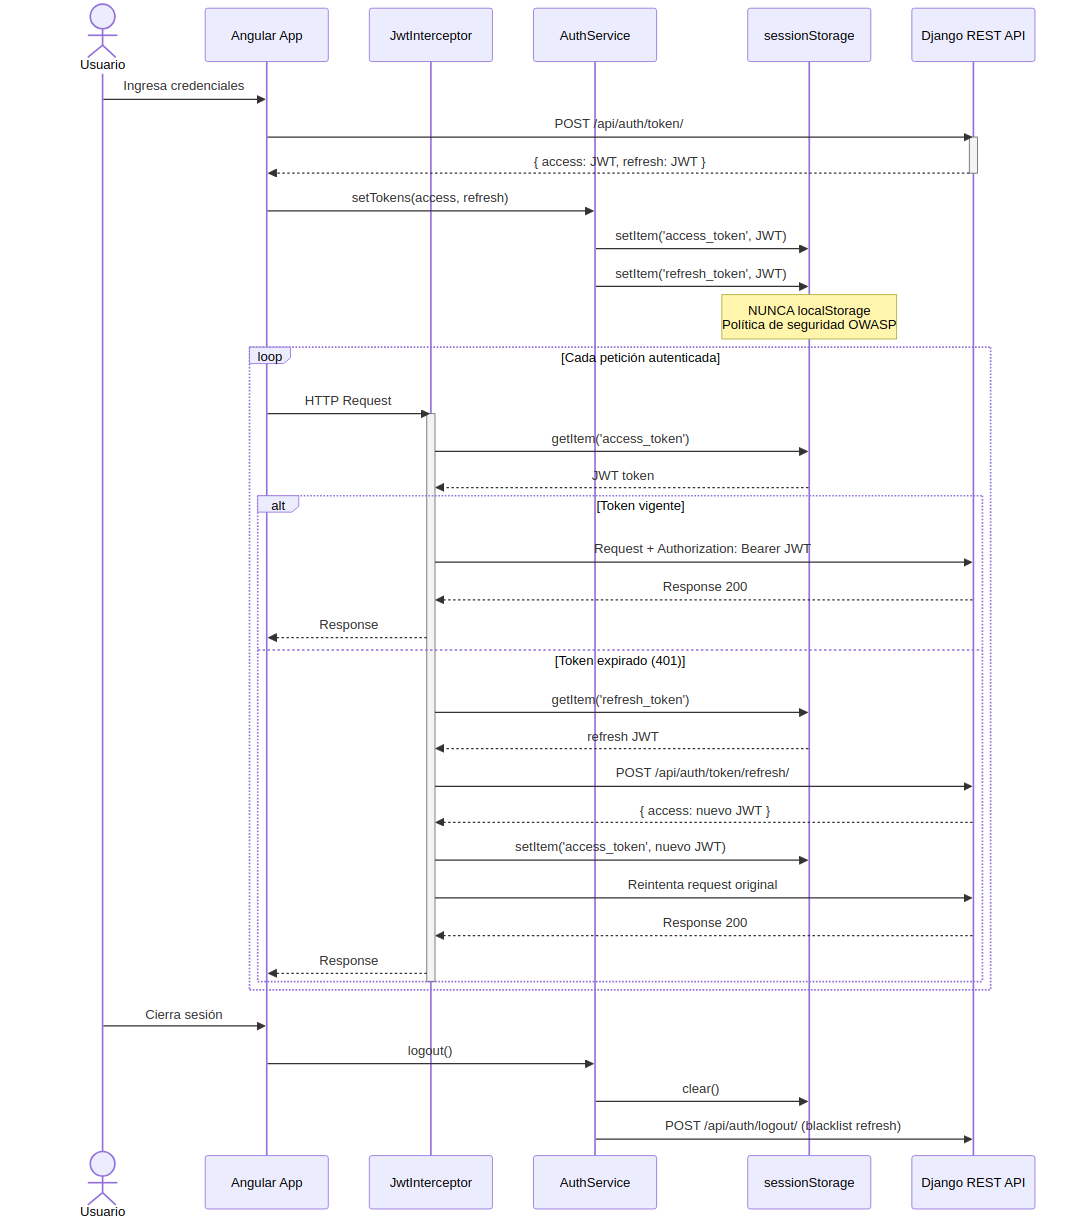
\includegraphics[width=0.92\textwidth]{../diagrams/generated/04_gestion_jwt_sesion.png}
  \caption{Ciclo de vida del JWT: autenticación, renovación automática y cierre de sesión}
  \label{fig:jwt}
\end{figure}

% ────────────────────────────────────────────────────────────────────────────
\section{Esquema de Base de Datos (ERD)}
% ────────────────────────────────────────────────────────────────────────────

\subsection{Descripción}

El modelo de datos refleja las entidades del dominio: usuarios con roles,
perfiles de artistas, solicitudes de cotización, citas y consentimientos de salud.

\subsection{Relaciones principales}

\begin{tcolorbox}[infobox, title={Cardinalidades clave}]
\begin{itemize}[itemsep=4pt]
  \item \textbf{User (STUDIO)} $\to$ \textbf{ArtistProfile:} relación 1:1
  \item \textbf{User (CLIENT)} $\to$ \textbf{QuoteRequest:} relación 1:N
  \item \textbf{ArtistProfile} $\leftrightarrow$ \textbf{TattooStyle:} M:N (artista domina varios estilos)
  \item \textbf{QuoteRequest} $\to$ \textbf{Appointment:} 1:N (un quote puede generar múltiples citas)
  \item \textbf{Appointment} $\to$ \textbf{HealthConsent:} 1:1 (opcional hasta que se aprueba la cita)
\end{itemize}
\end{tcolorbox}

\subsection{Diagrama entidad-relación}

\begin{figure}[H]
  \centering
  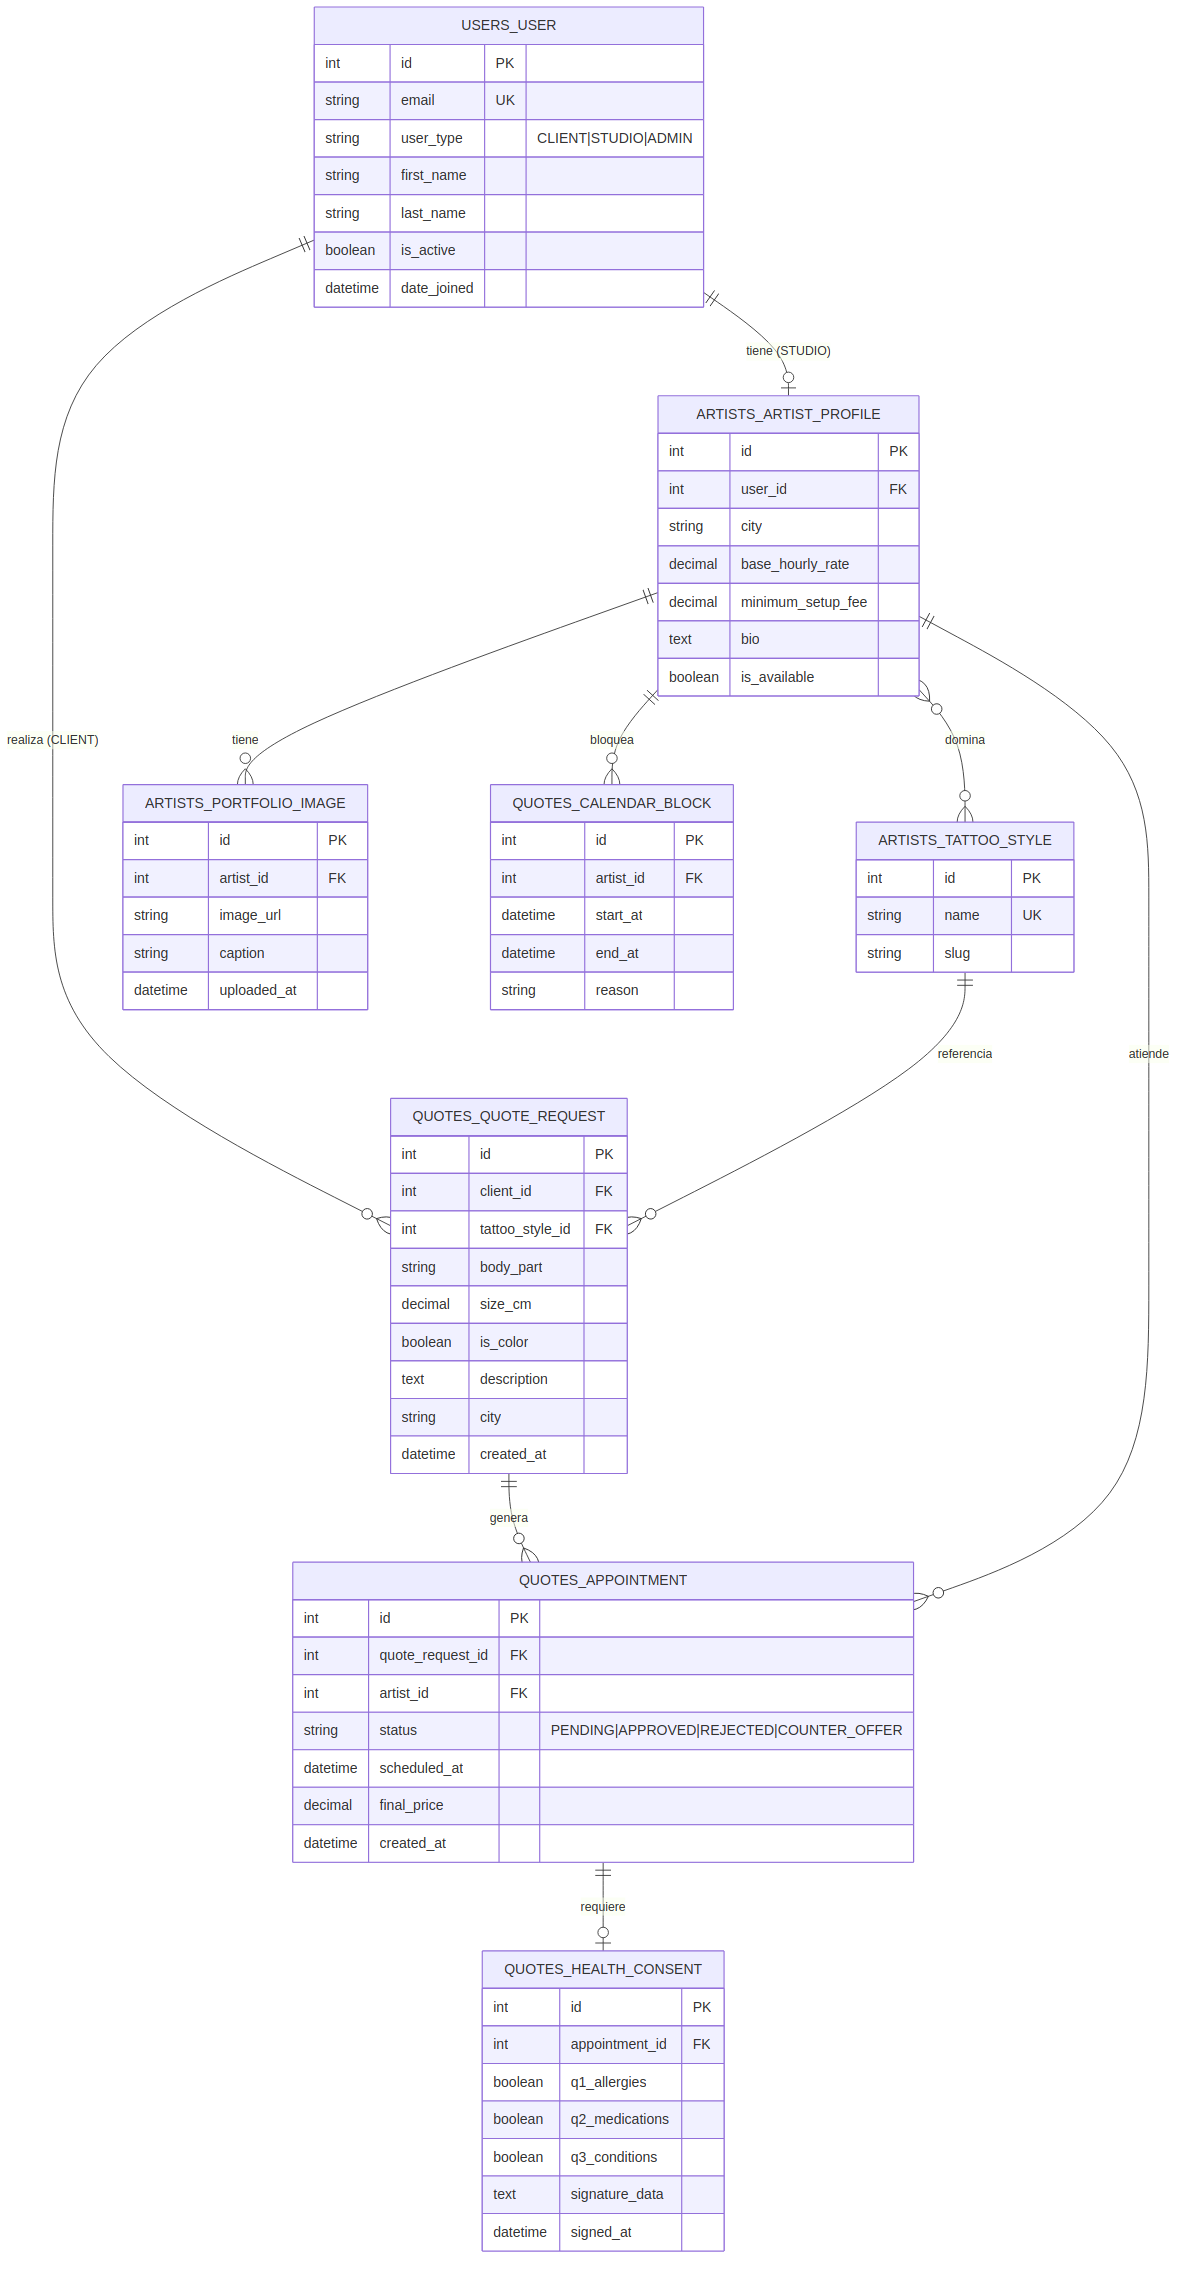
\includegraphics[width=0.95\textwidth]{../diagrams/generated/05_erd_base_datos.png}
  \caption{Diagrama entidad-relación del esquema BlackLine en PostgreSQL}
  \label{fig:erd}
\end{figure}

% ────────────────────────────────────────────────────────────────────────────
\section{Normalización de Ciudades}
% ────────────────────────────────────────────────────────────────────────────

\subsection{Descripción}

La normalización de ciudades garantiza que el matching artista-cliente funcione
con búsquedas exactas. El catálogo \texttt{cities-mx.ts} es la fuente de verdad compartida
entre frontend y backend.

\subsection{Problema que resuelve}

Sin normalización, un cliente que escribe ``Gdl'' o ``guadalajara'' no encontraría
artistas registrados como ``Guadalajara''. El catálogo y el filtro \texttt{city\_\_iexact}
garantizan coincidencias exactas independientemente de mayúsculas/minúsculas.

\subsection{Invariantes del sistema}

\begin{tcolorbox}[rulebox, title={Reglas de normalización (siempre vigentes)}]
\begin{enumerate}[itemsep=4pt]
  \item Usar \textbf{siempre} el catálogo \texttt{frontend/src/app/core/data/cities-mx.ts}
  \item \textbf{Nunca} texto libre en campos de ciudad
  \item Backend filtra con \texttt{city\_\_iexact} — el catálogo garantiza la coincidencia
  \item \textbf{Pendiente (backlog):} migrar \texttt{ArtistProfile.city} a FK hacia tabla normalizada
\end{enumerate}
\end{tcolorbox}

\subsection{Diagrama de flujo}

\begin{figure}[H]
  \centering
  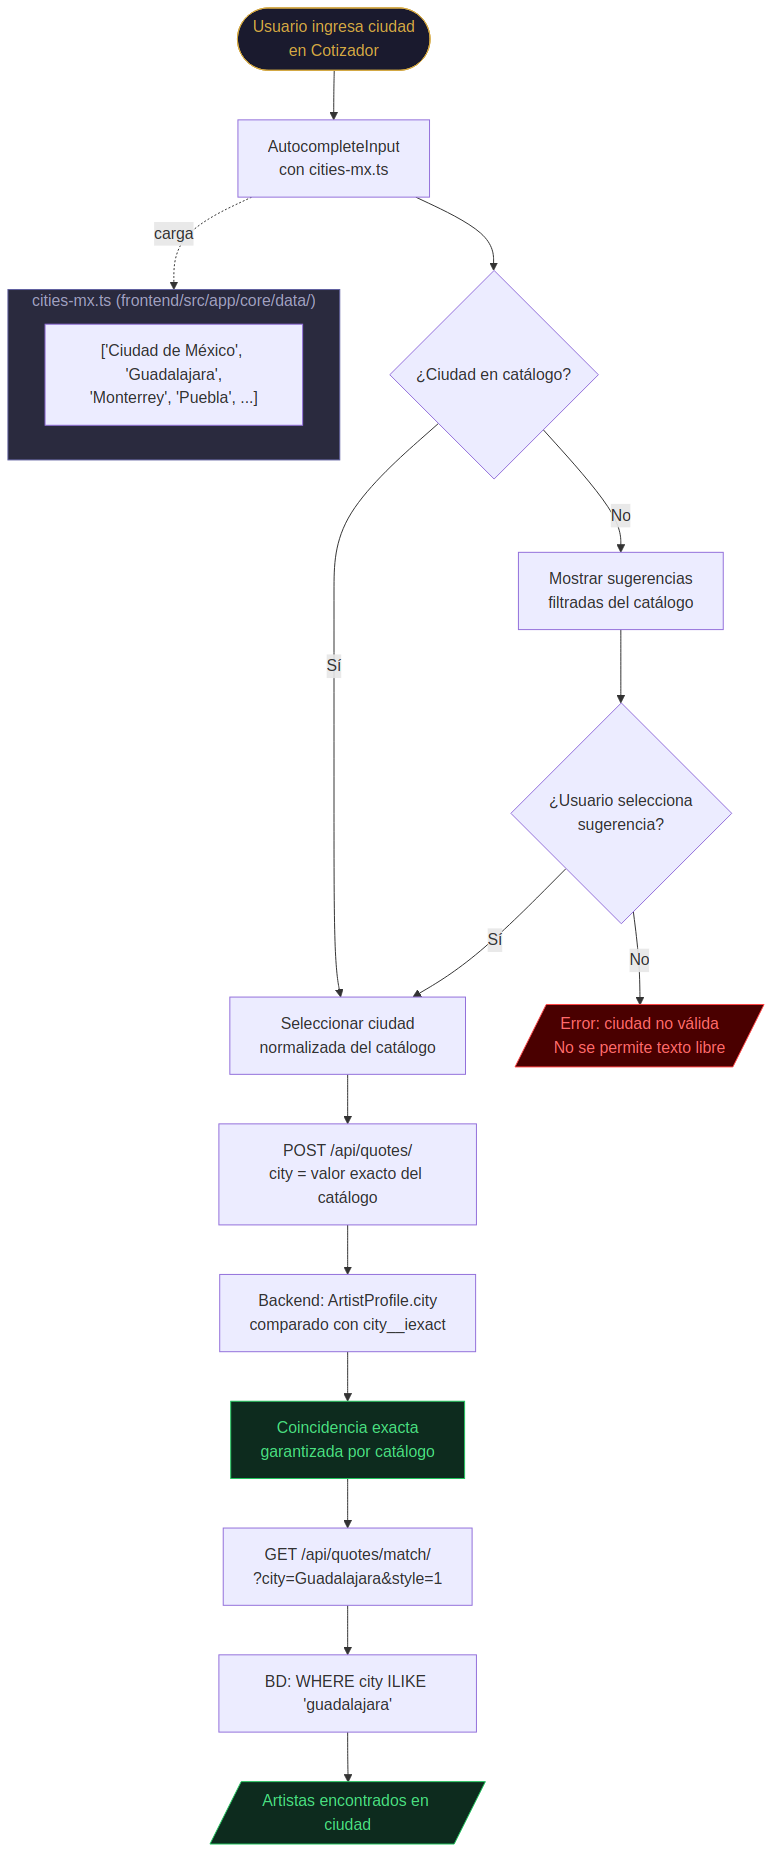
\includegraphics[width=0.78\textwidth]{../diagrams/generated/06_normalizacion_ciudades.png}
  \caption{Flujo de normalización de ciudades desde el Cotizador hasta el filtro de Match}
  \label{fig:ciudades}
\end{figure}

% ────────────────────────────────────────────────────────────────────────────
\section{Flujo de Contraoferta de Precio y Fecha (BL-95-RF-4)}
% ────────────────────────────────────────────────────────────────────────────

\subsection{Descripción}

Cuando un artista no puede aceptar la cita en los términos propuestos por el cliente,
puede emitir una \textbf{contraoferta} con una nueva fecha y/o nota explicativa.
El cliente entonces puede aceptar (transición a \texttt{APPROVED}) pero no rechazar —
la única transición válida desde \texttt{COUNTER\_OFFER} es \texttt{APPROVED}.

\subsection{Validaciones del serializer}

\begin{tcolorbox}[codebox, title={AppointmentStatusSerializer — regla de contraoferta}]
\texttt{class AppointmentStatusSerializer(serializers.Serializer):}\\
\texttt{\ \ \ \ status = ChoiceField(choices=Appointment.Status.choices)}\\
\texttt{\ \ \ \ counter\_offer\_datetime = DateTimeField(required=False, allow\_null=True)}\\
\texttt{\ \ \ \ counter\_offer\_note = CharField(required=False, default="", allow\_blank=True)}\\[6pt]
\texttt{\ \ \ \ def validate(self, data):}\\
\texttt{\ \ \ \ \ \ \ \ if data["status"] == "COUNTER\_OFFER":}\\
\texttt{\ \ \ \ \ \ \ \ \ \ \ \ if not data.get("counter\_offer\_datetime"):}\\
\texttt{\ \ \ \ \ \ \ \ \ \ \ \ \ \ \ \ raise ValidationError(\{"counter\_offer\_datetime": "Requerido."\})}
\end{tcolorbox}

\begin{center}
\begin{tabular}{lll}
\toprule
\rowcolor{blkMid}
\textcolor{blkGold}{\textbf{Estado origen}} &
\textcolor{blkGold}{\textbf{Estado destino}} &
\textcolor{blkGold}{\textbf{Actor / Restricción}}\\
\midrule
\texttt{PENDING}       & \texttt{COUNTER\_OFFER} & Artista dueño de la cita + \texttt{counter\_offer\_datetime} requerida\\
\rowcolor{blkMid}
\texttt{PENDING}       & \texttt{APPROVED}       & Artista dueño de la cita\\
\texttt{PENDING}       & \texttt{REJECTED}       & Artista dueño de la cita\\
\rowcolor{blkMid}
\texttt{COUNTER\_OFFER}& \texttt{APPROVED}       & Solo el cliente — única transición válida\\
\texttt{COUNTER\_OFFER}& \texttt{REJECTED}       & \textcolor{blkRed}{\textbf{NO PERMITIDO}} → 400 Bad Request\\
\bottomrule
\end{tabular}
\end{center}

\begin{tcolorbox}[warnbox, title={Restricción implementada en views.py}]
Desde \texttt{COUNTER\_OFFER} el código retorna \texttt{400} si el cliente intenta
pasar a \texttt{REJECTED}. Solo \texttt{APPROVED} es válido desde ese estado.
Esta restricción es más estricta que la tabla de estados del §4.
\end{tcolorbox}

\subsection{Diagrama de secuencia}

\begin{figure}[H]
  \centering
  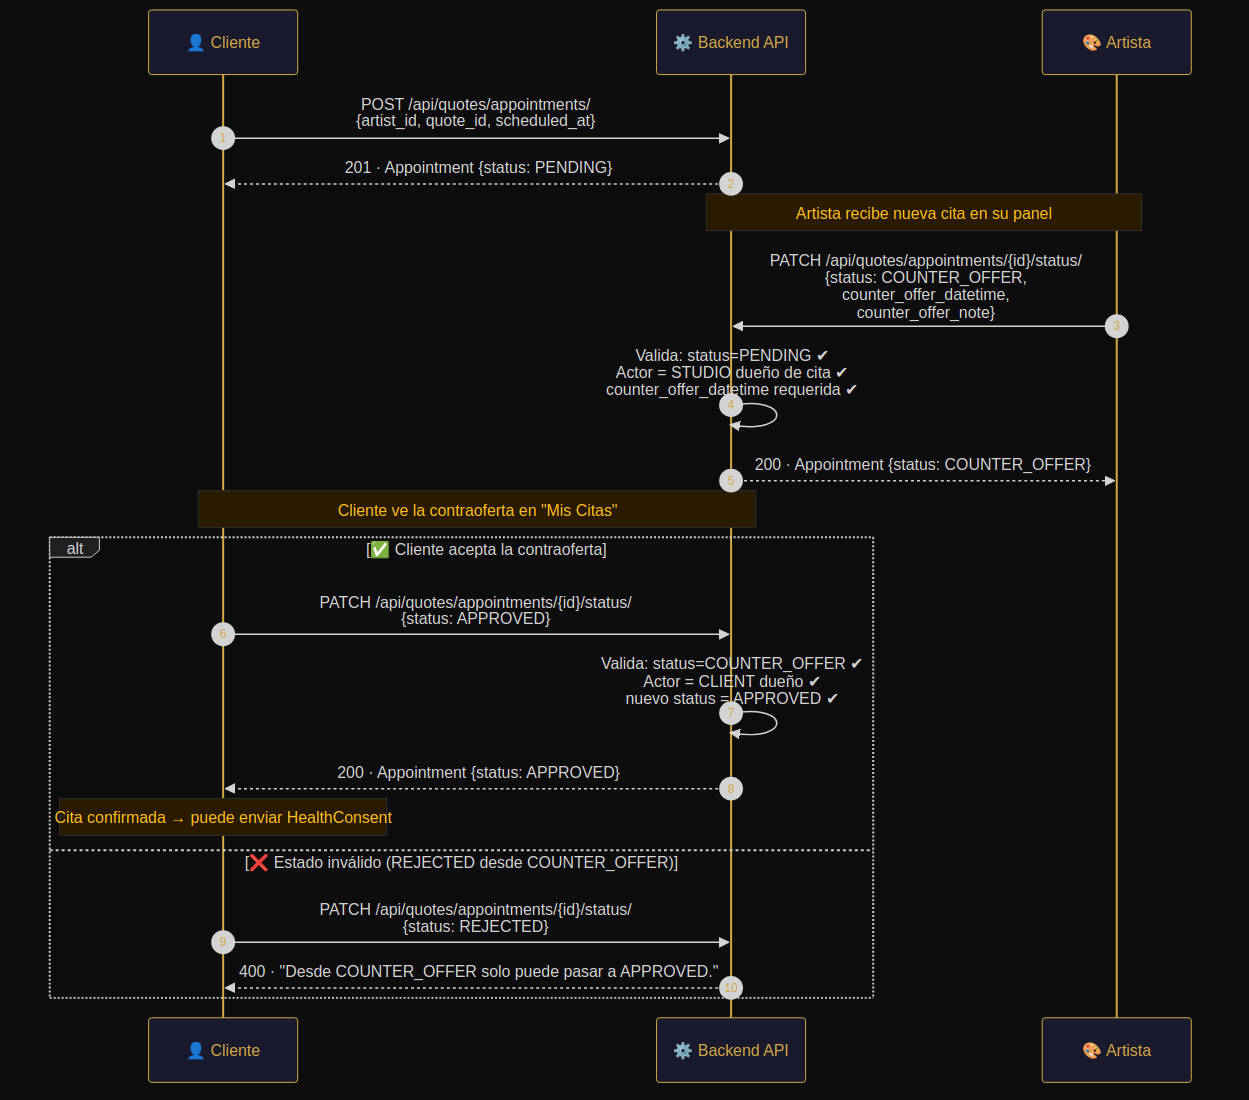
\includegraphics[width=0.95\textwidth]{../diagrams/generated/07_contraoferta_precio_fecha.png}
  \caption{Secuencia de contraoferta: artista propone cambios, cliente acepta o recibe error}
  \label{fig:contraoferta}
\end{figure}

% ────────────────────────────────────────────────────────────────────────────
\section{Validación de Solapamiento en CalendarBlock}
% ────────────────────────────────────────────────────────────────────────────

\subsection{Descripción}

El modelo \texttt{CalendarBlock} permite al artista bloquear franjas de tiempo.
La validación de solapamiento garantiza que no existan dos bloques simultáneos
ni que un bloqueo cubra una cita ya confirmada.

\subsection{Algoritmo de detección}

El solapamiento entre dos rangos \texttt{(A\_start, A\_end)} y \texttt{(B\_start, B\_end)}
existe si y solo si:
\[
A\_start < B\_end \;\wedge\; A\_end > B\_start
\]

Traducido a ORM de Django:

\begin{tcolorbox}[codebox, title={Query de detección de solapamiento (a agregar en CalendarBlockSerializer)}]
\texttt{\# Bloques existentes que se solapan con el nuevo rango}\\
\texttt{overlapping = CalendarBlock.objects.filter(}\\
\texttt{\ \ \ \ artist=artist,}\\
\texttt{\ \ \ \ start\_datetime\_\_lt=end\_datetime,}\\
\texttt{\ \ \ \ end\_datetime\_\_gt=start\_datetime,}\\
\texttt{)}\\[6pt]
\texttt{\# Citas APPROVED en ese rango}\\
\texttt{blocked = Appointment.objects.filter(}\\
\texttt{\ \ \ \ artist=artist,}\\
\texttt{\ \ \ \ status=Appointment.Status.APPROVED,}\\
\texttt{\ \ \ \ scheduled\_at\_\_gte=start\_datetime,}\\
\texttt{\ \ \ \ scheduled\_at\_\_lt=end\_datetime,}\\
\texttt{)}
\end{tcolorbox}

\subsection{Casos borde}

\begin{tcolorbox}[infobox, title={Casos límite del algoritmo}]
\begin{itemize}[itemsep=4pt]
  \item \textbf{Bloques contiguos:} \texttt{(08:00–10:00)} y \texttt{(10:00–12:00)} \textbf{no} se solapan
    porque $10{:}00 \not< 10{:}00$.
  \item \textbf{Mismo horario exacto:} \texttt{(08:00–10:00)} y \texttt{(08:00–10:00)} \textbf{sí} se solapan.
  \item \textbf{Bloqueo parcial:} \texttt{(09:00–11:00)} sobre \texttt{(08:00–10:00)} \textbf{sí} se solapa.
  \item El método \texttt{CalendarBlock.full\_clean()} ya valida que \texttt{start < end} antes de guardar.
\end{itemize}
\end{tcolorbox}

\subsection{Diagrama de decisión}

\begin{figure}[H]
  \centering
  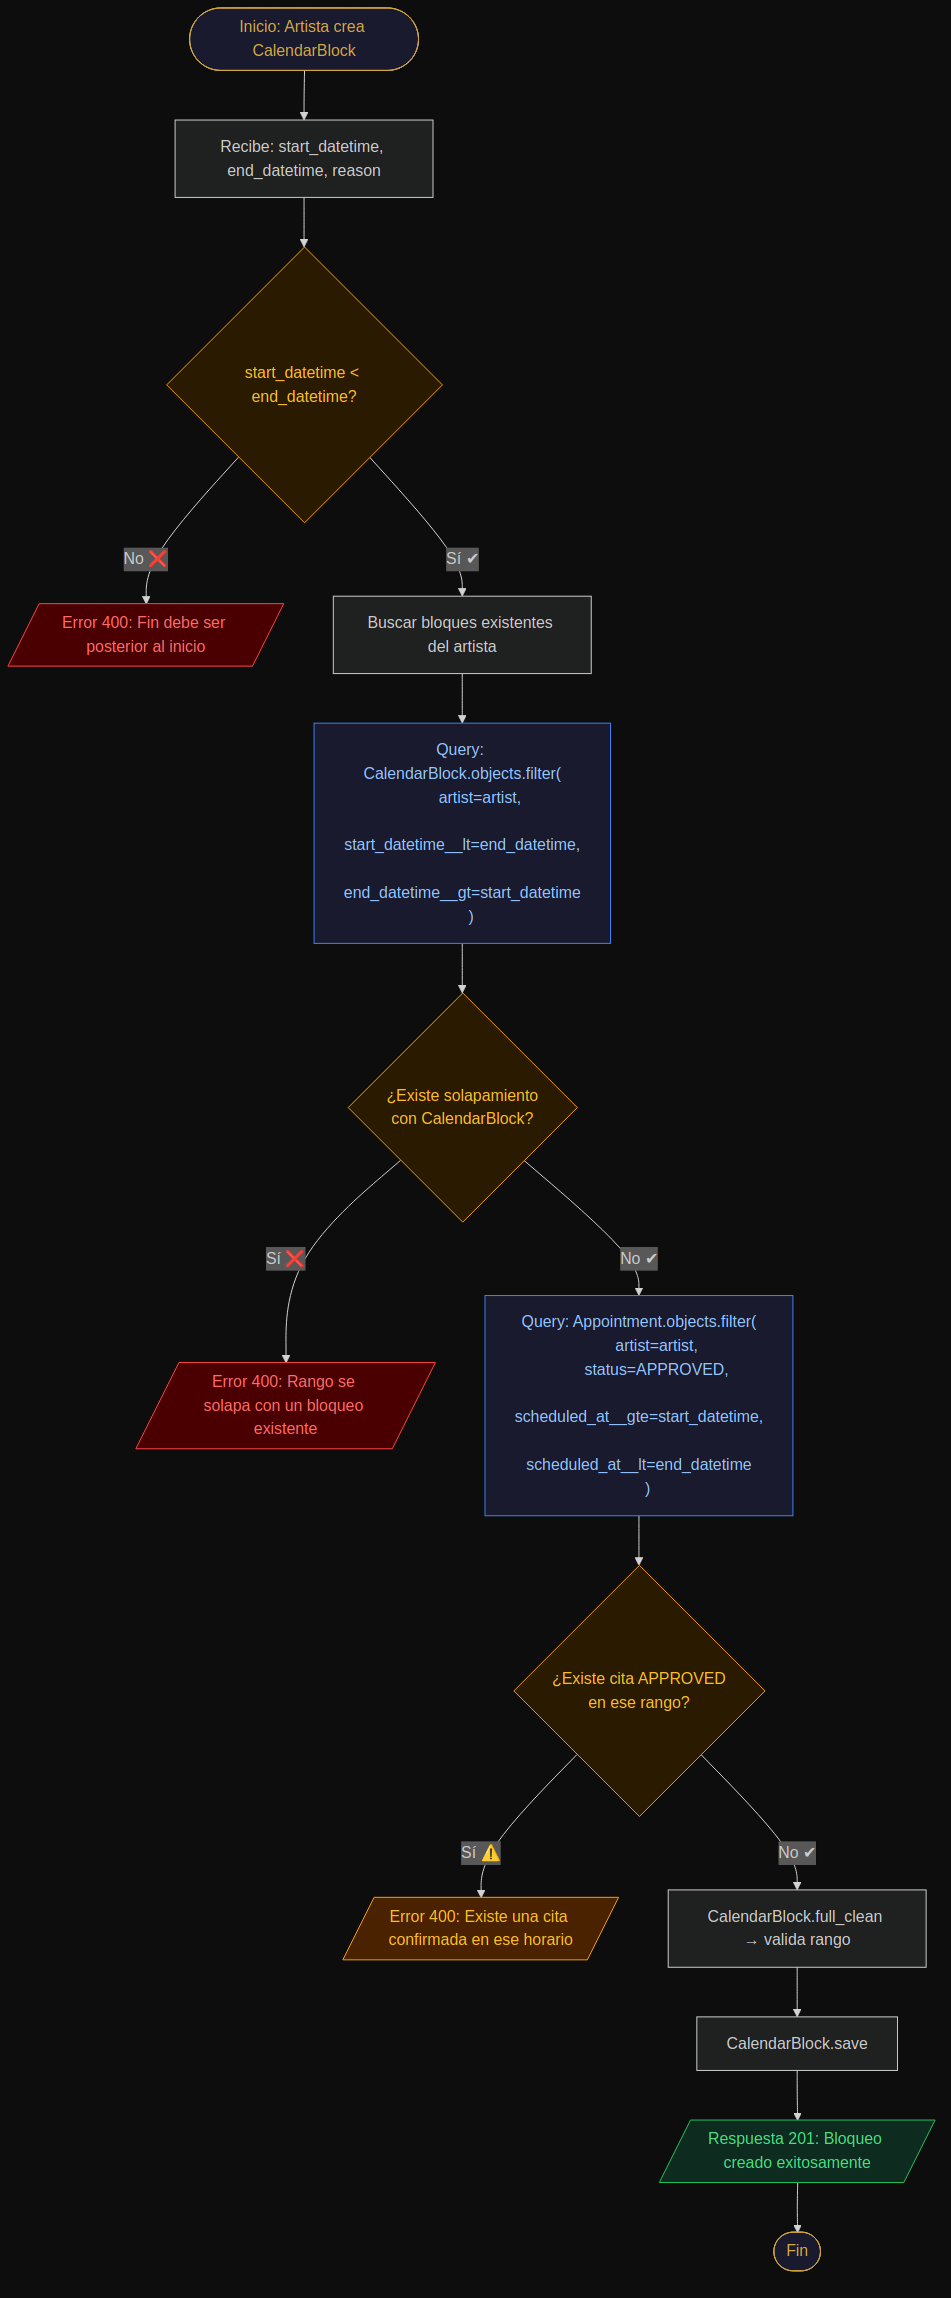
\includegraphics[width=0.88\textwidth]{../diagrams/generated/08_validacion_solapamiento_calendario.png}
  \caption{Algoritmo de validación de solapamiento en CalendarBlock (pendiente de implementar)}
  \label{fig:solapamiento}
\end{figure}

% ────────────────────────────────────────────────────────────────────────────
\section{Pipeline OpenAPI $\to$ Tipos Angular}
% ────────────────────────────────────────────────────────────────────────────

\subsection{Descripción}

El contrato API se sincroniza automáticamente entre backend y frontend mediante
el pipeline \textbf{drf-spectacular → openapi-typescript}. Saltarse este paso
produce drift silencioso: los tipos TypeScript quedan desactualizados sin error.

\subsection{Cuándo regenerar}

\begin{tcolorbox}[warnbox, title={Obligatorio regenerar si cambia cualquiera de estos}]
\begin{itemize}[itemsep=3pt]
  \item Un serializer (campo nuevo, renombrado o eliminado)
  \item Un ViewSet o APIView (método, endpoint, parámetro)
  \item Un \texttt{@extend\_schema} o decorador de drf-spectacular
  \item Un modelo cuyos campos se exponen directamente en un serializer
\end{itemize}
\end{tcolorbox}

\subsection{Comandos del pipeline}

\begin{tcolorbox}[codebox, title={Paso 1 — Generar schema.yml (backend)}]
\texttt{cd backend}\\
\texttt{python manage.py spectacular --file schema.yml}
\end{tcolorbox}

\begin{tcolorbox}[codebox, title={Paso 2 — Regenerar tipos TypeScript (frontend)}]
\texttt{cd \$PROJECT\_ROOT}\\
\texttt{npx openapi-typescript backend/schema.yml \textbackslash}\\
\texttt{\ \ -o frontend/src/app/core/api/types.ts}
\end{tcolorbox}

\begin{tcolorbox}[codebox, title={Paso 3 — Detectar drift antes del PR}]
\texttt{git diff backend/schema.yml}\\
\texttt{\# Si hay cambios, también debe haber diff en frontend/src/app/core/api/types.ts}
\end{tcolorbox}

\subsection{Diagrama de dependencias}

\begin{figure}[H]
  \centering
  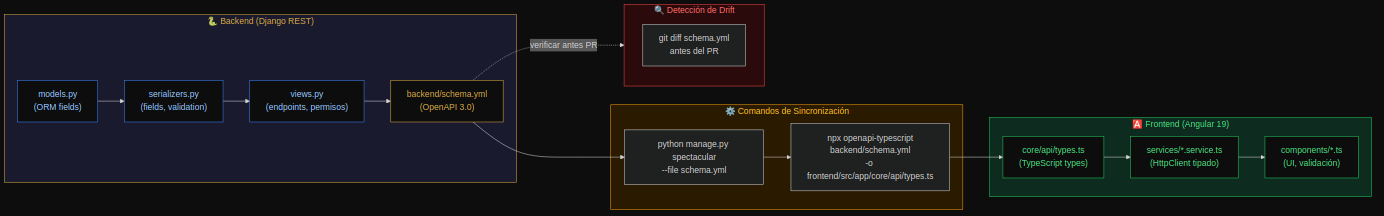
\includegraphics[width=0.95\textwidth]{../diagrams/generated/09_pipeline_openapi_tipos.png}
  \caption{Pipeline de sincronización: models.py → schema.yml → types.ts → componentes Angular}
  \label{fig:openapi}
\end{figure}

% ────────────────────────────────────────────────────────────────────────────
\section{Flujo de Cuestionario de Salud (HealthConsent)}
% ────────────────────────────────────────────────────────────────────────────

\subsection{Descripción}

El cuestionario de salud es un \textbf{requisito legal} bajo la Ley Federal de
Protección de Datos Personales en Posesión de Particulares (LFPDPPP, México).
Solo puede enviarse una vez por cita y requiere firma digital del cliente.

\subsection{Campos del modelo}

\begin{center}
\begin{tabularx}{0.95\textwidth}{lXl}
\toprule
\rowcolor{blkMid}
\textcolor{blkGold}{\textbf{Campo}} &
\textcolor{blkGold}{\textbf{Descripción}} &
\textcolor{blkGold}{\textbf{Obligatorio}}\\
\midrule
\texttt{has\_allergies} & ¿Tiene alergias? + detalle & No\\
\rowcolor{blkMid}
\texttt{has\_chronic\_disease} & Diabetes, hipertensión, coagulopatías & No\\
\texttt{takes\_medication} & Anticoagulantes, corticosteroides, etc. & No\\
\rowcolor{blkMid}
\texttt{is\_pregnant} & Embarazo o lactancia & No\\
\texttt{has\_skin\_condition} & Psoriasis, queloide, dermatitis & No\\
\rowcolor{blkMid}
\texttt{has\_hemophilia} & Trastorno de coagulación & No\\
\texttt{signature\_data} & PNG del cliente en base64 (\texttt{data:image/png;base64,...}) & \textbf{Sí}\\
\rowcolor{blkMid}
\texttt{terms\_accepted} & Aceptación LFPDPPP & \textbf{Sí}\\
\bottomrule
\end{tabularx}
\end{center}

\begin{tcolorbox}[warnbox, title={Reglas de negocio (LFPDPPP)}]
\begin{itemize}[itemsep=3pt]
  \item \textbf{Idempotencia:} el endpoint \texttt{POST} rechaza si ya existe un consent para esa cita (400).
  \item \textbf{Firma obligatoria:} \texttt{signature\_data} debe iniciar con \texttt{"data:image/"}.
  \item \textbf{Términos obligatorios:} \texttt{terms\_accepted = false} → 400.
  \item \textbf{Solo el cliente:} actores \texttt{STUDIO} o \texttt{ADMIN} reciben 403.
  \item \textbf{Retención:} los datos se almacenan indefinidamente por cumplimiento legal.
\end{itemize}
\end{tcolorbox}

\subsection{Diagrama de secuencia}

\begin{figure}[H]
  \centering
  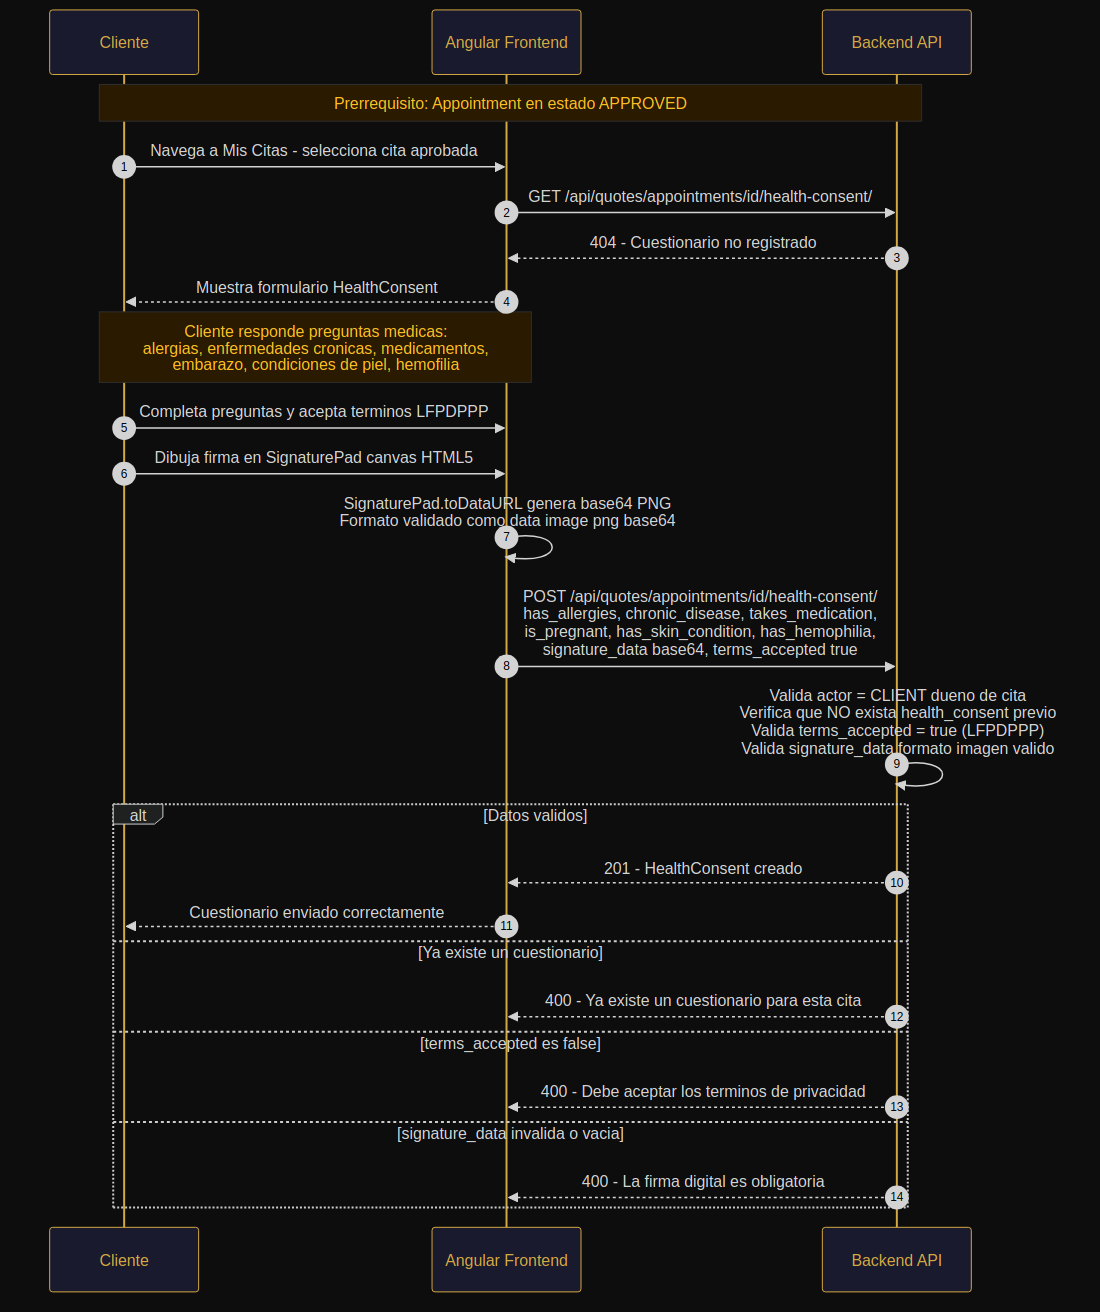
\includegraphics[width=0.95\textwidth]{../diagrams/generated/10_flujo_health_consent.png}
  \caption{Flujo completo de HealthConsent: firma digital → validaciones LFPDPPP → persistencia}
  \label{fig:health}
\end{figure}

% ────────────────────────────────────────────────────────────────────────────
\section{Algoritmo de Match (Filtrado de Artistas)}
% ────────────────────────────────────────────────────────────────────────────

\subsection{Descripción}

El endpoint \texttt{GET /api/quotes/match/} es el corazón del marketplace.
Todo el cálculo de precio estimado se ejecuta en \textbf{una sola query SQL}
mediante \texttt{annotate} del ORM de Django, cumpliendo el RNF-2 ($\leq 2.5$\,s de respuesta).

\subsection{Parámetros de entrada}

\begin{center}
\begin{tabular}{llll}
\toprule
\rowcolor{blkMid}
\textcolor{blkGold}{\textbf{Parámetro}} &
\textcolor{blkGold}{\textbf{Tipo}} &
\textcolor{blkGold}{\textbf{Obligatorio}} &
\textcolor{blkGold}{\textbf{Descripción}}\\
\midrule
\texttt{city}      & string  & Sí & Ciudad del artista (iexact)\\
\rowcolor{blkMid}
\texttt{style\_id} & integer & Sí & PK del estilo deseado\\
\texttt{size\_cm}  & integer & Sí & Tamaño estimado en cm ($\geq 1$)\\
\rowcolor{blkMid}
\texttt{body\_part}& choice  & Sí & Zona del cuerpo\\
\texttt{is\_color} & boolean & Sí & ¿A color?\\
\rowcolor{blkMid}
\texttt{max\_price}& decimal & No & Presupuesto máximo del cliente\\
\bottomrule
\end{tabular}
\end{center}

\subsection{Pipeline de la query (7 pasos)}

\begin{tcolorbox}[codebox, title={SQL compilado por el ORM — ArtistMatchView.get()}]
\texttt{SELECT id, city, bio, base\_hourly\_rate, minimum\_setup\_fee,}\\
\texttt{\ \ GREATEST(}\\
\texttt{\ \ \ \ \{size\_cm\} * base\_hourly\_rate * \{zone\_mult\} * \{clr\_mult\},}\\
\texttt{\ \ \ \ minimum\_setup\_fee}\\
\texttt{\ \ ) AS estimated\_price,}\\
\texttt{\ \ CASE WHEN styles.id = \{style\_id\} THEN TRUE ELSE FALSE END AS style\_match}\\
\texttt{FROM artists\_artistprofile}\\
\texttt{JOIN users\_user ON user\_id = users\_user.id}\\
\texttt{WHERE users\_user.is\_active = TRUE}\\
\texttt{\ \ AND base\_hourly\_rate > 0}\\
\texttt{\ \ AND minimum\_setup\_fee > 0}\\
\texttt{\ \ AND city ILIKE '\{city\}'}\\
\texttt{ORDER BY style\_match DESC, estimated\_price ASC}
\end{tcolorbox}

\begin{tcolorbox}[infobox, title={Criterios que faltan (backlog)}]
El Match actual \textbf{no filtra} por \texttt{CalendarBlock} ni por \texttt{Appointment} aprobadas
en la fecha deseada. Un artista con agenda llena aparecerá igual en los resultados.
Pendiente: agregar parámetro \texttt{desired\_date} y excluir artistas bloqueados.
\end{tcolorbox}

\subsection{Diagrama de flujo}

\begin{figure}[H]
  \centering
  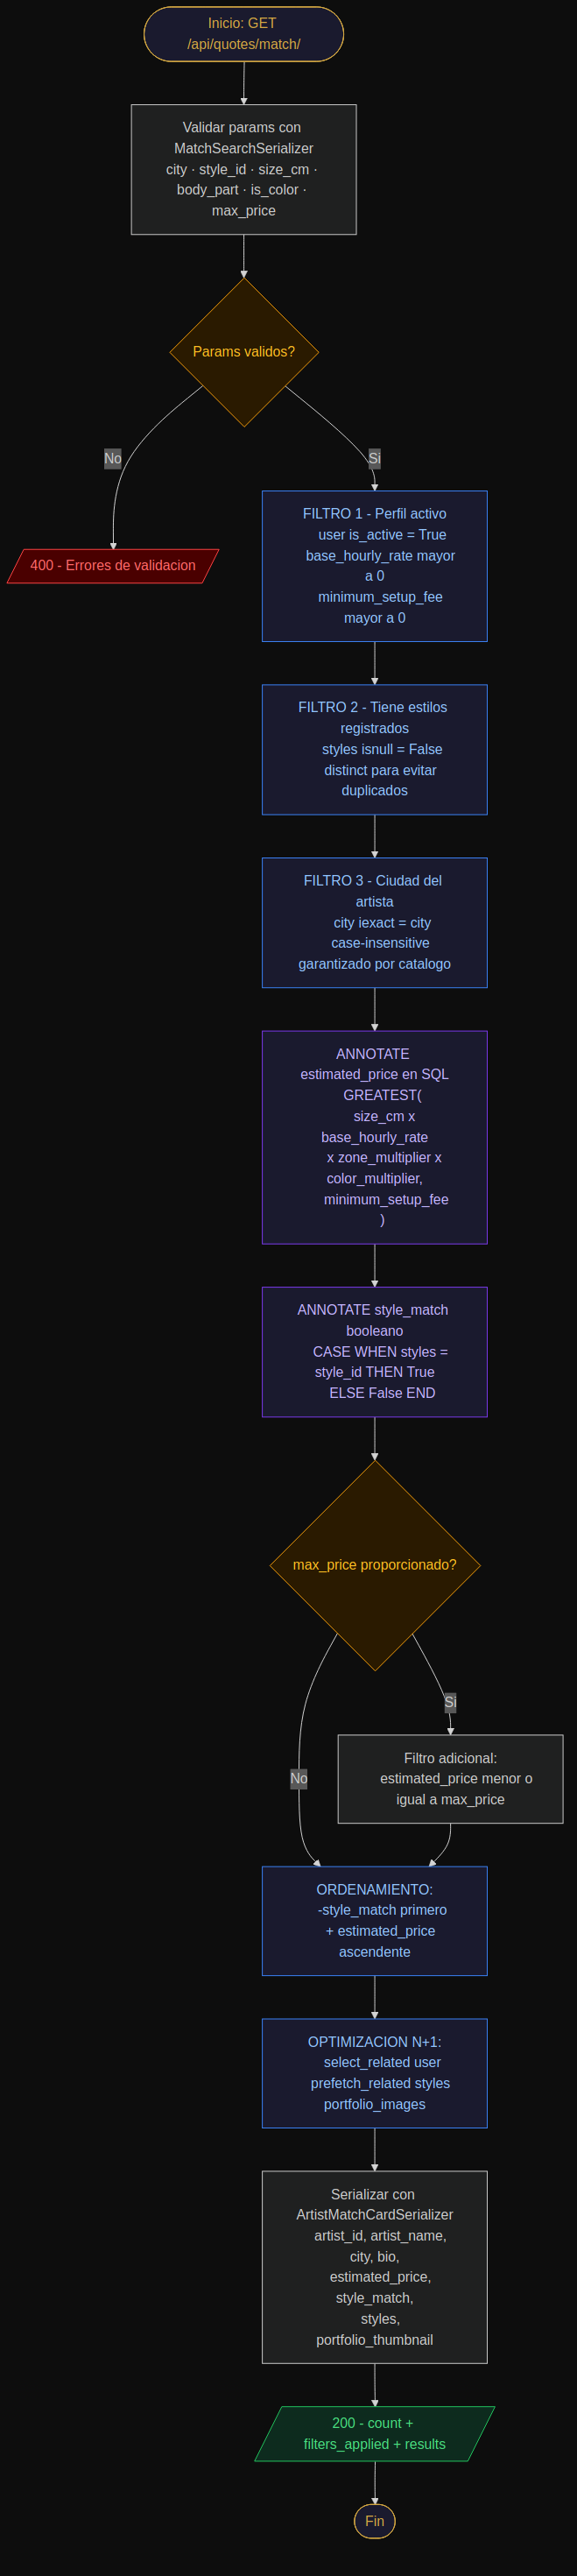
\includegraphics[width=0.90\textwidth]{../diagrams/generated/11_algoritmo_match.png}
  \caption{Pipeline completo del motor de matchmaking en 7 pasos — una sola query SQL}
  \label{fig:match}
\end{figure}

% ────────────────────────────────────────────────────────────────────────────
\section{Guards y Permisos por Rol (Angular)}
% ────────────────────────────────────────────────────────────────────────────

\subsection{Descripción}

La aplicación implementa tres guards funcionales (\texttt{CanActivateFn}) que protegen
las rutas según el estado de autenticación y el rol del usuario.

\subsection{Guards implementados}

\begin{tcolorbox}[codebox, title={authGuard — Verifica sesión activa}]
\texttt{// Comprueba:}\\
\texttt{// 1. Existe user en memoria}\\
\texttt{// 2. Access token en sessionStorage + no expirado (exp × 1000 > Date.now())}\\
\texttt{// Si falla → redirige a /auth/login?returnUrl=\{ruta\_original\}}
\end{tcolorbox}

\begin{tcolorbox}[codebox, title={roleGuard(…roles) — Verifica rol específico}]
\texttt{roleGuard('CLIENT')   // Solo clientes}\\
\texttt{roleGuard('STUDIO')   // Solo artistas}\\
\texttt{// ADMIN pasa siempre (bypass de roles)}\\
\texttt{// Rol incorrecto → redirige al dashboard del rol real}
\end{tcolorbox}

\begin{tcolorbox}[codebox, title={noAuthGuard — Rutas públicas}]
\texttt{// Si ya hay sesión activa → redirectByRole():}\\
\texttt{//   STUDIO → /studio/dashboard}\\
\texttt{//   CLIENT → /client/dashboard}\\
\texttt{//   ADMIN  → /admin/ (Django Admin, fuera de la SPA)}\\
\texttt{// Evita que usuarios logueados vean landing/login}
\end{tcolorbox}

\subsection{Árbol de rutas protegidas}

\begin{center}
\begin{tabular}{lll}
\toprule
\rowcolor{blkMid}
\textcolor{blkGold}{\textbf{Ruta}} &
\textcolor{blkGold}{\textbf{Guards}} &
\textcolor{blkGold}{\textbf{Roles permitidos}}\\
\midrule
\texttt{/} (landing) & \texttt{noAuthGuard} & Sin sesión\\
\rowcolor{blkMid}
\texttt{/auth/**} & — & Público (no guard)\\
\texttt{/client/**} & \texttt{authGuard + roleGuard('CLIENT')} & CLIENT, ADMIN\\
\rowcolor{blkMid}
\texttt{/studio/**} & \texttt{authGuard + roleGuard('STUDIO')} & STUDIO, ADMIN\\
\bottomrule
\end{tabular}
\end{center}

\subsection{Diagrama de flujo}

\begin{figure}[H]
  \centering
  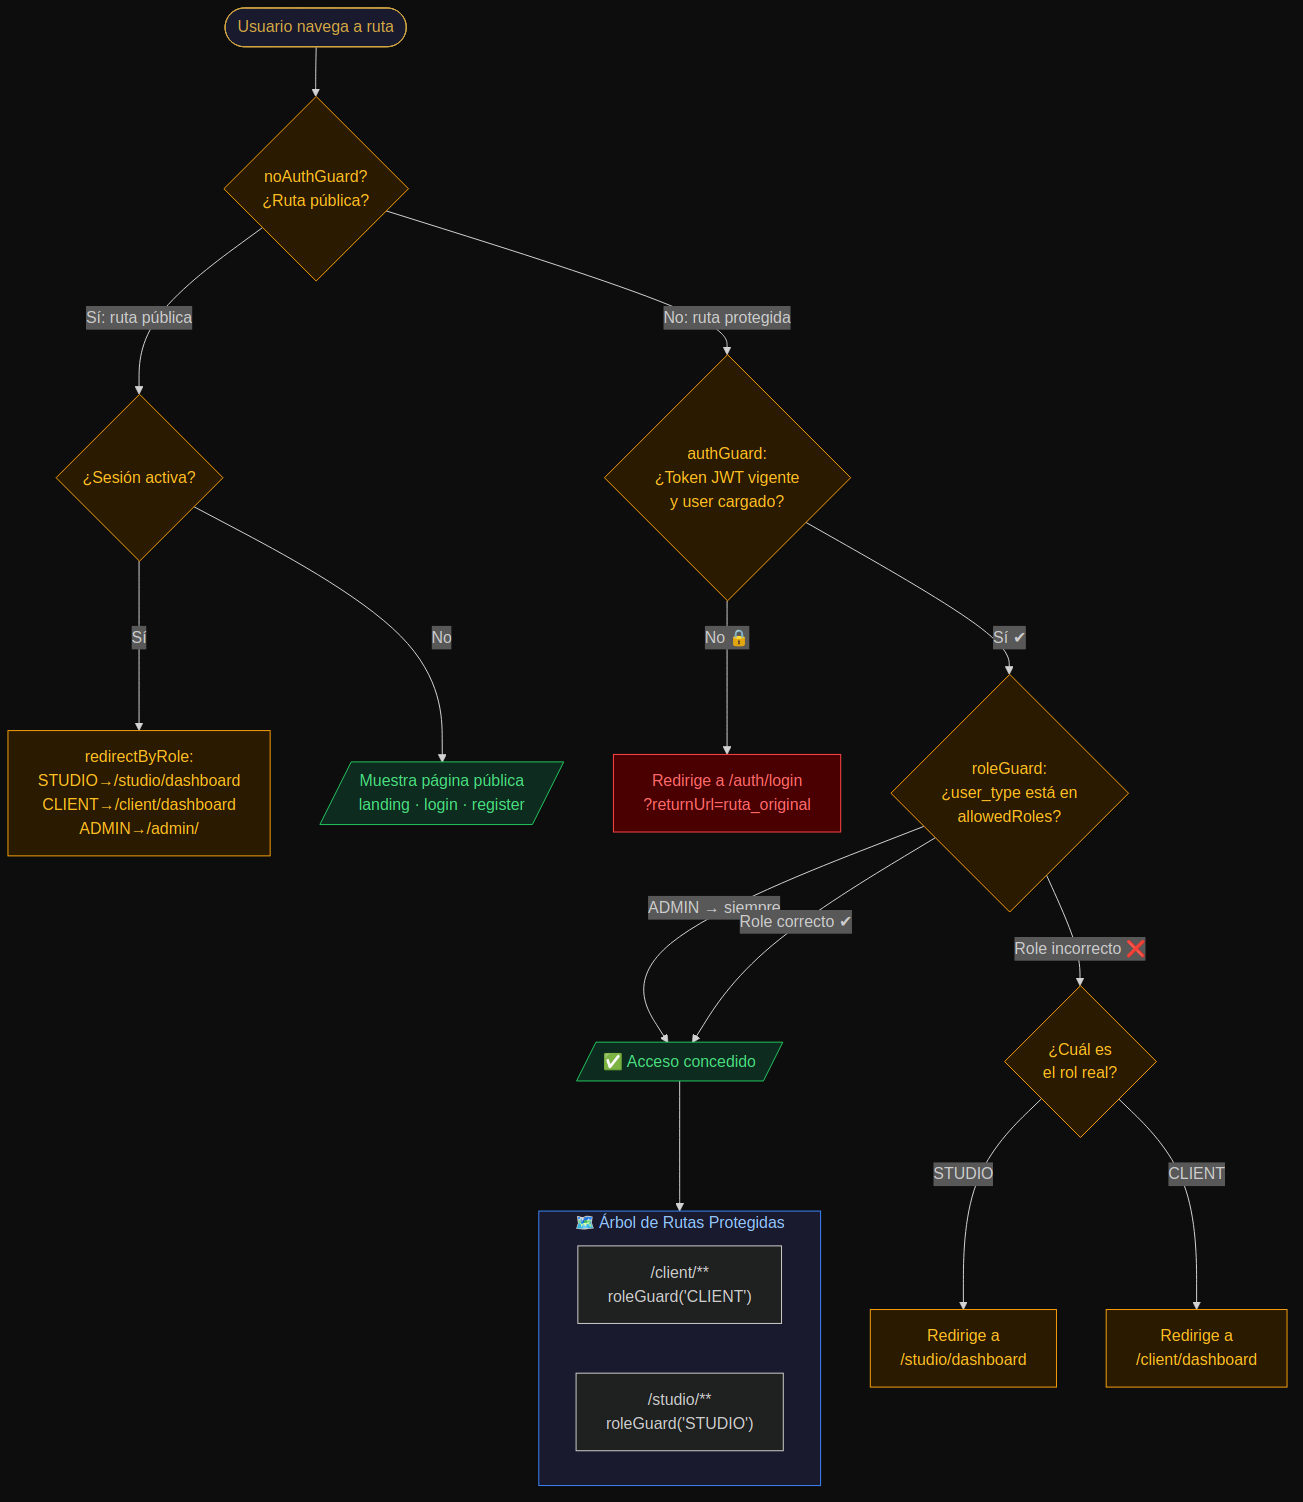
\includegraphics[width=0.90\textwidth]{../diagrams/generated/12_guards_permisos_angular.png}
  \caption{Árbol de decisión de los guards Angular: noAuth → auth → role}
  \label{fig:guards}
\end{figure}

% ────────────────────────────────────────────────────────────────────────────
\section{Permisos DRF en el Backend}
% ────────────────────────────────────────────────────────────────────────────

\subsection{Descripción}

Cada endpoint del backend verifica \textbf{autenticación + rol + propiedad del recurso}.
La función auxiliar \texttt{\_get\_appointment\_or\_403} centraliza la lógica de ownership.

\subsection{Tabla de permisos por endpoint}

\begin{center}
\begin{tabularx}{\textwidth}{llX}
\toprule
\rowcolor{blkMid}
\textcolor{blkGold}{\textbf{Endpoint}} &
\textcolor{blkGold}{\textbf{Método}} &
\textcolor{blkGold}{\textbf{Quien puede}}\\
\midrule
\texttt{/api/quotes/} & GET & CLIENT (sus quotes)\\
\rowcolor{blkMid}
\texttt{/api/quotes/} & POST & CLIENT\\
\texttt{/api/quotes/match/} & GET & \textbf{Público} (\texttt{AllowAny})\\
\rowcolor{blkMid}
\texttt{/api/quotes/appointments/} & GET & CLIENT (las suyas) · STUDIO (las suyas) · ADMIN (todas)\\
\texttt{/api/quotes/appointments/} & POST & Solo CLIENT\\
\rowcolor{blkMid}
\texttt{/api/quotes/appointments/\{id\}/status/} & PATCH & STUDIO (desde PENDING) · CLIENT (desde COUNTER\_OFFER)\\
\texttt{/api/quotes/appointments/\{id\}/health-consent/} & POST & Solo CLIENT dueño\\
\rowcolor{blkMid}
\texttt{/api/quotes/calendar-blocks/} & GET & STUDIO (los suyos) · ADMIN (todos)\\
\texttt{/api/quotes/calendar-blocks/} & POST & Solo STUDIO\\
\rowcolor{blkMid}
\texttt{/api/quotes/calendar-blocks/\{id\}/} & DELETE & Solo STUDIO dueño\\
\bottomrule
\end{tabularx}
\end{center}

\begin{tcolorbox}[warnbox, title={Escalada de privilegios — riesgos y mitigaciones}]
\begin{itemize}[itemsep=3pt]
  \item Un \texttt{STUDIO} intenta cambiar estado de cita de otro artista → 403 (verificado con \texttt{appt.artist.user != user}).
  \item Un \texttt{CLIENT} intenta enviar COUNTER\_OFFER → 400 (verificado en la máquina de estados).
  \item Un \texttt{STUDIO} intenta crear una cita → 403 (\texttt{user\_type != "CLIENT"}).
  \item \textbf{Pendiente:} custom permission classes (\texttt{IsArtistOwner}, \texttt{IsClientOwner})
    para reemplazar los \texttt{if} inline y centralizar la lógica.
\end{itemize}
\end{tcolorbox}

\subsection{Diagrama de permisos}

\begin{figure}[H]
  \centering
  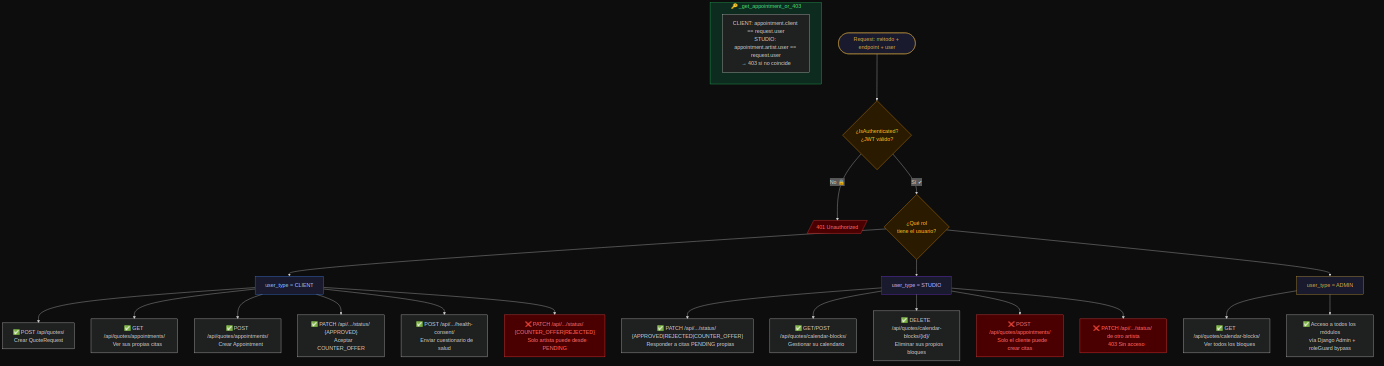
\includegraphics[width=0.95\textwidth]{../diagrams/generated/13_permisos_drf_backend.png}
  \caption{Árbol de permisos por rol: autenticación → rol → ownership del recurso}
  \label{fig:permisos}
\end{figure}

% ────────────────────────────────────────────────────────────────────────────
\section{Cálculo del Rango de Precio en el Frontend}
% ────────────────────────────────────────────────────────────────────────────

\subsection{Descripción}

El frontend calcula un rango de precio \textbf{estimado} usando una tarifa de mercado
promedio (\texttt{BASE\_RATE\_MXN = 150}) antes de que el cliente elija artista.
Este precio es orientativo; el precio definitivo lo calcula el backend con la
tarifa real del artista.

\subsection{Fórmula frontend}

\begin{tcolorbox}[codebox, title={cotizador.component.ts — \_calcPrice()}]
\texttt{const BASE\_RATE\_MXN = 150;  // MXN/cm — tarifa de mercado promedio}\\[6pt]
\texttt{function \_calcPrice(form): \{ min: number; max: number \} | null \{}\\
\texttt{\ \ const factor = ZONE\_MULTIPLIERS[form.body\_part];}\\
\texttt{\ \ const colorMult = form.is\_color ? 1.20 : 1.00;}\\
\texttt{\ \ const price = Math.round(}\\
\texttt{\ \ \ \ BASE\_RATE\_MXN * form.size\_cm * factor * colorMult / 10}\\
\texttt{\ \ ) * 10;}\\
\texttt{\ \ return \{ min: price, max: Math.round(price * 1.35 / 10) * 10 \};}\\
\texttt{\}}
\end{tcolorbox}

\subsection{Diferencia entre precio frontend y precio backend}

\begin{center}
\begin{tabularx}{0.95\textwidth}{lXX}
\toprule
\rowcolor{blkMid}
\textcolor{blkGold}{\textbf{}} &
\textcolor{blkGold}{\textbf{Frontend (estimado)}} &
\textcolor{blkGold}{\textbf{Backend (real)}}\\
\midrule
Tarifa base & \texttt{BASE\_RATE\_MXN = 150} (constante) & \texttt{ArtistProfile.base\_hourly\_rate} (por artista)\\
\rowcolor{blkMid}
Cuándo & Paso 3 del Cotizador (sin artista) & Resultado del Match (con artista)\\
Propósito & Orientar al cliente & Precio oficial de la tarjeta\\
\rowcolor{blkMid}
Fuente de verdad & No & \textbf{Sí}\\
\bottomrule
\end{tabularx}
\end{center}

\begin{tcolorbox}[warnbox, title={Riesgo de desincronización}]
\texttt{BASE\_RATE\_MXN = 150} es una constante arbitraria. Si el mercado sube,
el estimado del cotizador podría quedar muy por debajo del precio real del artista,
generando una expectativa incorrecta al cliente. Considerar obtenerlo desde un
endpoint de configuración o como promedio dinámico.
\end{tcolorbox}

\subsection{Diagrama de flujo}

\begin{figure}[H]
  \centering
  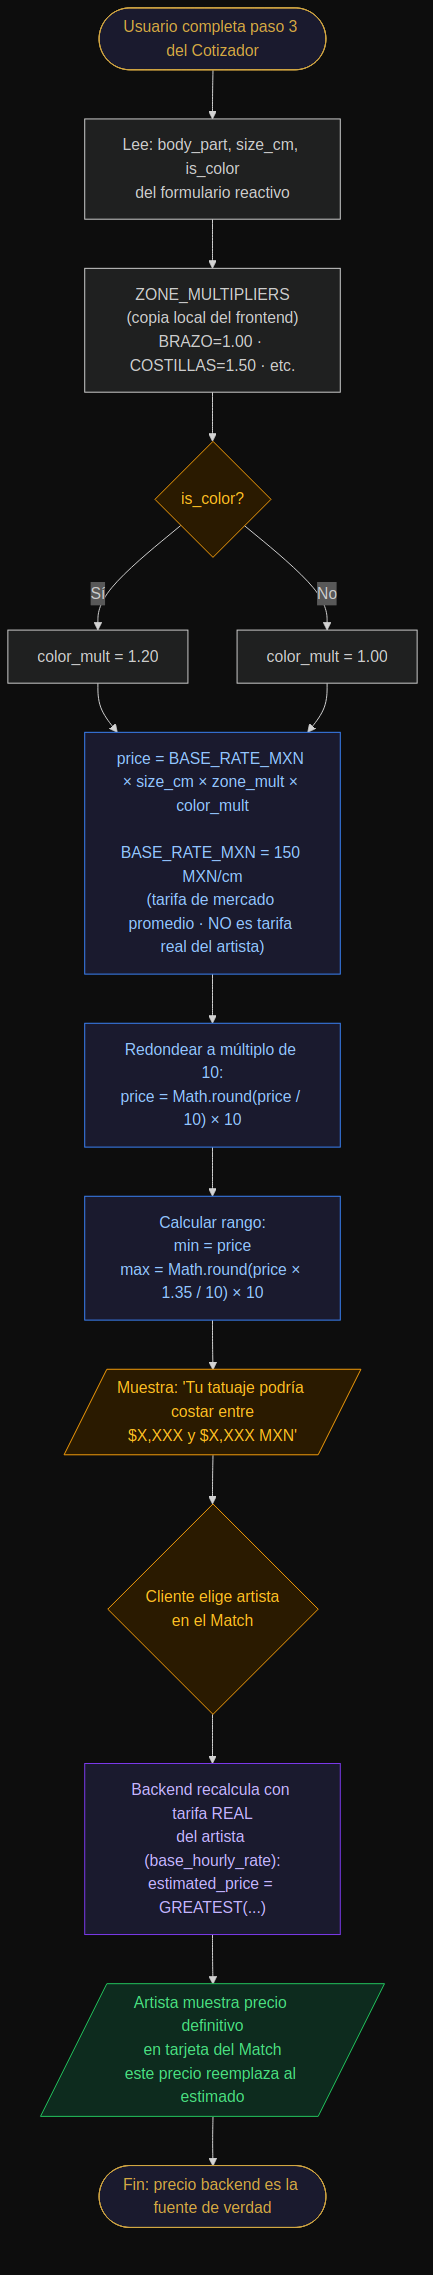
\includegraphics[width=0.85\textwidth]{../diagrams/generated/14_rango_precio_frontend.png}
  \caption{Cálculo del rango estimado en frontend vs. precio real calculado en backend}
  \label{fig:rangoprecio}
\end{figure}

% ────────────────────────────────────────────────────────────────────────────
\section{Índices de Base de Datos (Performance)}
% ────────────────────────────────────────────────────────────────────────────

\subsection{Descripción}

Sin índices adecuados, las queries de Match y listado de citas degradarán con
el volumen de datos. Los índices que se describen a continuación están priorizados
por impacto estimado.

\subsection{Índices recomendados}

\begin{center}
\begin{tabularx}{\textwidth}{lXl}
\toprule
\rowcolor{blkMid}
\textcolor{blkGold}{\textbf{Modelo}} &
\textcolor{blkGold}{\textbf{Índice}} &
\textcolor{blkGold}{\textbf{Prioridad}}\\
\midrule
\texttt{QuoteRequest} & \texttt{(client\_id, created\_at DESC)} & Alta\\
\rowcolor{blkMid}
\texttt{Appointment} & \texttt{(artist\_id, status, scheduled\_at)} & Alta\\
\texttt{Appointment} & \texttt{(artist\_id, scheduled\_at) WHERE status='APPROVED'} & Alta\\
\rowcolor{blkMid}
\texttt{CalendarBlock} & \texttt{(artist\_id, start\_datetime, end\_datetime)} & Media\\
\texttt{ArtistProfile} & \texttt{(city)} & Media (afecta Match)\\
\bottomrule
\end{tabularx}
\end{center}

\subsection{Implementación con migraciones Django}

\begin{tcolorbox}[codebox, title={Agregar en Meta de los modelos}]
\texttt{class Meta:}\\
\texttt{\ \ indexes = [}\\
\texttt{\ \ \ \ models.Index(}\\
\texttt{\ \ \ \ \ \ fields=["client", "-created\_at"],}\\
\texttt{\ \ \ \ \ \ name="qr\_client\_created\_idx",}\\
\texttt{\ \ \ \ ),}\\
\texttt{\ \ \ \ models.Index(}\\
\texttt{\ \ \ \ \ \ fields=["artist", "status", "scheduled\_at"],}\\
\texttt{\ \ \ \ \ \ name="appt\_artist\_status\_idx",}\\
\texttt{\ \ \ \ ),}\\
\texttt{\ \ ]}
\end{tcolorbox}

\begin{tcolorbox}[codebox, title={Índice parcial con RunSQL (solo APPROVED)}]
\texttt{migrations.RunSQL(}\\
\texttt{\ \ "CREATE INDEX appt\_approved\_idx ON quotes\_appointment}\\
\texttt{\ \ \ (artist\_id, scheduled\_at) WHERE status = 'APPROVED';",}\\
\texttt{\ \ reverse\_sql="DROP INDEX IF EXISTS appt\_approved\_idx;",}\\
\texttt{)}
\end{tcolorbox}

\subsection{Diagrama de índices}

\begin{figure}[H]
  \centering
  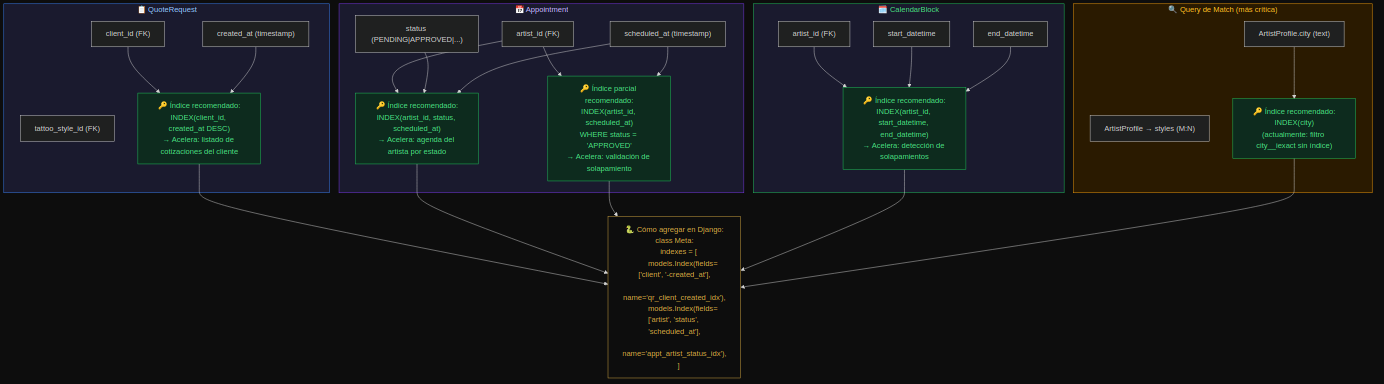
\includegraphics[width=0.92\textwidth]{../diagrams/generated/15_indices_base_datos.png}
  \caption{Índices recomendados por tabla e impacto en las queries críticas}
  \label{fig:indices}
\end{figure}

% ────────────────────────────────────────────────────────────────────────────
\section{Endpoint GET /api/quotes/cities/ (Backlog UX)}
% ────────────────────────────────────────────────────────────────────────────

\subsection{Descripción}

Actualmente el autocomplete de ciudades en el Match usa el catálogo estático
\texttt{cities-mx.ts} con todas las ciudades de México. Este endpoint retornaría
solo las ciudades donde hay artistas activos, mejorando la UX al no mostrar
ciudades sin cobertura.

\subsection{Implementación propuesta}

\begin{tcolorbox}[codebox, title={Query del endpoint (backend/apps/quotes/views.py)}]
\texttt{class ActiveCitiesView(APIView):}\\
\texttt{\ \ permission\_classes = [AllowAny]}\\[4pt]
\texttt{\ \ def get(self, request):}\\
\texttt{\ \ \ \ cities = (}\\
\texttt{\ \ \ \ \ \ ArtistProfile.objects}\\
\texttt{\ \ \ \ \ \ .filter(user\_\_is\_active=True, base\_hourly\_rate\_\_gt=0)}\\
\texttt{\ \ \ \ \ \ .values\_list("city", flat=True)}\\
\texttt{\ \ \ \ \ \ .distinct()}\\
\texttt{\ \ \ \ \ \ .order\_by("city")}\\
\texttt{\ \ \ \ )}\\
\texttt{\ \ \ \ return Response(\{"cities": list(cities)\})}
\end{tcolorbox}

\begin{tcolorbox}[infobox, title={Estrategia de caché (Redis)}]
Este endpoint puede cachearse agresivamente porque las ciudades activas cambian
raramente:
\begin{itemize}[itemsep=3pt]
  \item \textbf{TTL recomendado:} 1 hora (3\,600 s)
  \item \textbf{Invalidación:} al activar/desactivar un \texttt{ArtistProfile}
  \item \textbf{Implementación:} \texttt{@method\_decorator(cache\_page(3600))} o caché manual con Django-Redis
\end{itemize}
\end{tcolorbox}

\subsection{Integración con el autocomplete Angular}

\begin{tcolorbox}[codebox, title={Intersección de catálogos en el componente Match}]
\texttt{// 1. Cargar ciudades activas del backend}\\
\texttt{const activeCities = await this.citiesService.getActiveCities();}\\[4pt]
\texttt{// 2. Filtrar el catálogo estático cities-mx.ts}\\
\texttt{const availableCities = CITIES\_MX.filter(c => activeCities.includes(c));}\\[4pt]
\texttt{// 3. Solo mostrar ciudades con cobertura en el autocomplete}\\
\texttt{this.filteredCities = availableCities;}
\end{tcolorbox}

\subsection{Diagrama de flujo}

\begin{figure}[H]
  \centering
  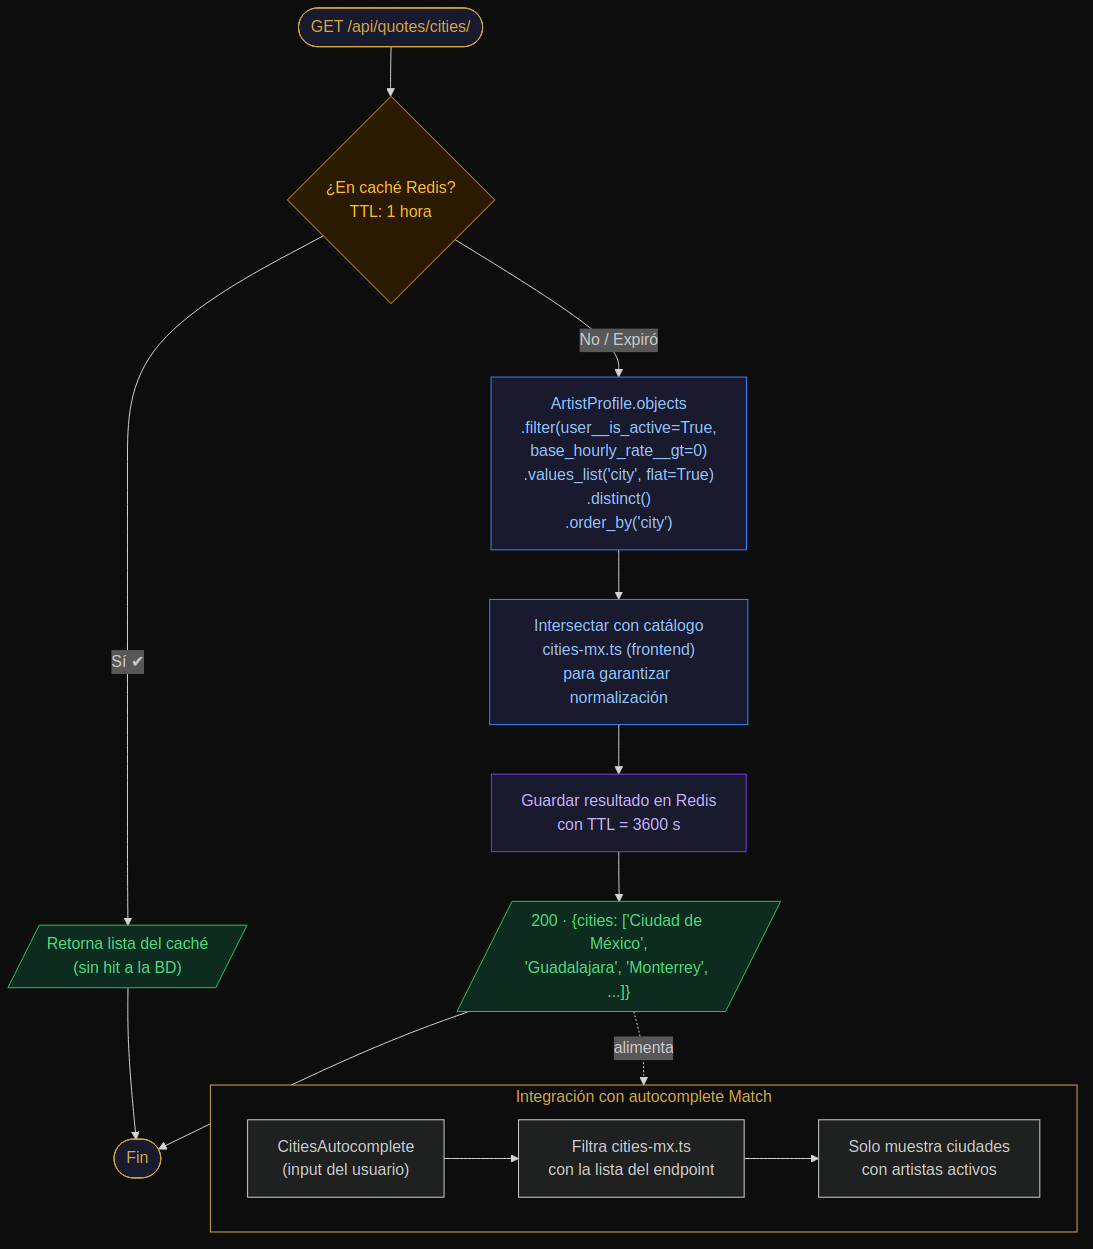
\includegraphics[width=0.85\textwidth]{../diagrams/generated/16_endpoint_cities.png}
  \caption{Endpoint de ciudades activas con caché Redis e integración con autocomplete Angular}
  \label{fig:cities}
\end{figure}

% ────────────────────────────────────────────────────────────────────────────
\section{Resumen de Endpoints Críticos}
% ────────────────────────────────────────────────────────────────────────────

\begin{center}
\begin{tabularx}{\textwidth}{llX}
\toprule
\rowcolor{blkMid}
\textcolor{blkGold}{\textbf{Método}} &
\textcolor{blkGold}{\textbf{Endpoint}} &
\textcolor{blkGold}{\textbf{Descripción}}\\
\midrule
\texttt{POST} & \texttt{/api/auth/token/} & Login, retorna access + refresh JWT\\
\rowcolor{blkMid}
\texttt{POST} & \texttt{/api/auth/token/refresh/} & Renueva access token\\
\texttt{POST} & \texttt{/api/quotes/} & Crea QuoteRequest (4 pasos cotizador)\\
\rowcolor{blkMid}
\texttt{GET}  & \texttt{/api/quotes/match/} & Artistas disponibles por ciudad+estilo\\
\texttt{POST} & \texttt{/api/quotes/appointments/} & Agenda cita (PENDING)\\
\rowcolor{blkMid}
\texttt{PATCH}& \texttt{/api/quotes/appointments/\{id\}/status/} & Cambia estado (artista)\\
\texttt{POST} & \texttt{/api/quotes/appointments/\{id\}/health-consent/} & Guarda consentimiento\\
\rowcolor{blkMid}
\texttt{GET}  & \texttt{/api/artists/styles/} & Catálogo de estilos de tatuaje\\
\rowcolor{blkMid}
\texttt{GET}  & \texttt{/api/quotes/calendar-blocks/} & Bloques de calendario del artista\\
\texttt{POST} & \texttt{/api/quotes/calendar-blocks/} & Artista bloquea franja de tiempo\\
\rowcolor{blkMid}
\texttt{DELETE}& \texttt{/api/quotes/calendar-blocks/\{id\}/} & Elimina un bloqueo\\
\texttt{GET}  & \texttt{/api/quotes/cities/} & \textit{(Backlog)} Ciudades con artistas activos\\
\bottomrule
\end{tabularx}
\end{center}

\vspace{1.5cm}

% ─── Tabla de estado de documentación ────────────────────────────────────────
\subsection*{Estado de la documentación}

\begin{center}
\begin{tabularx}{\textwidth}{Xlc}
\toprule
\rowcolor{blkMid}
\textcolor{blkGold}{\textbf{Algoritmo / Flujo}} &
\textcolor{blkGold}{\textbf{Sección}} &
\textcolor{blkGold}{\textbf{Estado}}\\
\midrule
Precio canónico (fórmula + multiplicadores)     & §2  & \textcolor{blkGreen}{✅}\\
\rowcolor{blkMid}
Flujo Cotizador → Match → Cita                  & §3  & \textcolor{blkGreen}{✅}\\
Máquina de estados de Appointment               & §4  & \textcolor{blkGreen}{✅}\\
\rowcolor{blkMid}
Gestión de sesión JWT + renovación automática   & §5  & \textcolor{blkGreen}{✅}\\
ERD de base de datos                            & §6  & \textcolor{blkGreen}{✅}\\
\rowcolor{blkMid}
Normalización de ciudades                       & §7  & \textcolor{blkGreen}{✅}\\
Flujo de Contraoferta (BL-95-RF-4)              & §8  & \textcolor{blkGreen}{✅}\\
\rowcolor{blkMid}
Validación de solapamiento CalendarBlock        & §9  & \textcolor{blkGreen}{✅}\\
Pipeline OpenAPI → Tipos Angular                & §10 & \textcolor{blkGreen}{✅}\\
\rowcolor{blkMid}
Flujo de HealthConsent (LFPDPPP)                & §11 & \textcolor{blkGreen}{✅}\\
Algoritmo de Match (7 pasos, SQL)               & §12 & \textcolor{blkGreen}{✅}\\
\rowcolor{blkMid}
Guards y permisos por rol (Angular)             & §13 & \textcolor{blkGreen}{✅}\\
Permisos DRF en el backend                      & §14 & \textcolor{blkGreen}{✅}\\
\rowcolor{blkMid}
Cálculo del rango de precio en frontend         & §15 & \textcolor{blkGreen}{✅}\\
Índices de base de datos (performance)          & §16 & \textcolor{blkGreen}{✅}\\
\rowcolor{blkMid}
Endpoint GET /api/quotes/cities/ (backlog)      & §17 & \textcolor{blkGreen}{✅}\\
\bottomrule
\end{tabularx}
\end{center}

\vspace{1.5cm}
\begin{center}
\textcolor{blkGold}{\rule{0.4\textwidth}{0.6pt}}\\[0.6cm]
{\small\color{blkText!50}
  BlackLine Engineering · Documentación técnica completa — v2.0.0\\
  \texttt{claude-sonnet-4-6} · Mayo 2026
}
\end{center}

\end{document}
